\documentclass[11pt,a4paper]{article}
\usepackage[utf8]{inputenc}
\usepackage[style=apa, backend=biber]{biblatex}
\usepackage[acronyms, toc]{glossaries}
\usepackage[ngerman]{babel}
\usepackage{csquotes}
\usepackage{graphicx}
\usepackage{geometry}
\usepackage{hyperref}
\usepackage{subfiles}
\usepackage{amssymb}
\usepackage{amsmath}
\usepackage{tabularx}
\usepackage{booktabs}
\usepackage{listings}
\usepackage{colortbl}
\usepackage{color}
\usepackage[rgb]{xcolor}
\usepackage{afterpage}
\usepackage{pdflscape}
\usepackage{tikz}
\usepackage{multicol}
\usepackage{enumitem}
\usepackage{float}


\geometry{a4paper, total={170mm,257mm}, left=20mm, top=20mm}
\usetikzlibrary{matrix, positioning, calc, fit, arrows.meta}

\newglossaryentry{wake-up-word}{
	name={Wake-up Wort},
	description={Ein Wake-up Wort ist ein Wort oder eine Wortsequenz, die ein System aktiviert.},
	plural={Wake-up Wörter}
}
\newacronym{ai}{AI}{Künstliche Intelligenz}



\newacronym{asr}{ASR}{Automatic Speech Recognition}
\newglossaryentry{automatic-speech-recognition}{
    name={Automatic Speech Recognition},
    description={Automatic Speech Recognition (ASR) ist die automatische Erkennung von Sprache.},
}

\newacronym{twd}{TWD}{Trigger Word Detection}
\newglossaryentry{trigger-word-detection}{
    name={Trigger Word Detection},
    description={Trigger Word Detection (TWD) ist die Erkennung eines bestimmten Wortes oder einer 
    bestimmten Wortsequenz.},
}
\makeglossaries
\renewcommand*{\glstextformat}[1]{\textit{#1}}
\renewcommand{\lstlistingname}{Source Code}

\addbibresource{references.bib}

\definecolor{ba-gray}{rgb}{0.9,0.9,0.9}
\definecolor{codeblack}{rgb}{0.1,0.1,0.23}
\definecolor{codegreen}{rgb}{0.2,0.5,0.1}
\definecolor{codepurple}{rgb}{0.5,0.0,0.5}
\definecolor{backcolour}{rgb}{0.95,0.95,0.95}
\definecolor{codered}{rgb}{0.7,0.1,0.2}

\lstset{
	language=Python,
	basicstyle=\ttfamily\footnotesize,
	backgroundcolor=\color{white},
	commentstyle=\color{codegreen},
	keywordstyle=\color{codered},
	numberstyle=\tiny\color{codegray},
	stringstyle=\color{codepurple},
	identifierstyle=\color{codeblack},
	showstringspaces=false,
	numbers=none,
	captionpos=b,
	frame=none,
	rulecolor=\color{black},
	aboveskip=1em, % Abstand über dem Code
	belowskip=1em  % Abstand unter dem Code
}


\title{
	{\LARGE Bachelorarbeit}\\[2em] 
	{\textbf{Integration von Sprachsteuerung {\break} in Mobile Apps}}
}

\author{Rubén Nuñez}
\date{Herbstsemester 2023}

\begin{document}

\maketitle
\thispagestyle{empty} %Keine Seitennummerierung auf der start Seite
\newpage

\section*{Bachelorarbeit an der Hochschule Luzern -- Informatik}
\subfile{affidavit.tex}
\newpage

% El sol es grande
\newpage \section*{Abstract}
Diese Bachelorarbeit konzentriert sich auf die Herausforderung, die Grundlage für eine integrierte 
Sprachsteuerung in mobilen Apps zu schaffen. Der Fokus liegt hierbei auf der Entwicklung einer 
Triggerwort-Erkennung, die es ermöglicht, bestimmte Wörter oder Wortsequenzen in der akustischen 
Sprache zu erkennen. Da integrierte Sprachsteuerungsfunktionen in mobilen Apps eher unüblich sind, 
bietet diese Arbeit eine innovative Lösung an. Der Ansatz umfasst drei Hauptkomponenten: die 
Erstellung eines ethisch und rechtlich einwandfreien Datensatzes, die Entwicklung und das Training 
eines effizienten Modells zur Erkennung von Triggerwörtern, und die Integration dieses Modells in 
eine mobile Anwendung.

\noindent \newline
Im Zentrum der Arbeit steht die Entwicklung eines Machine Learning-Modells, basierend auf einer 
Kombination aus Convolutional und Long-Short-Term-Memory (LSTM) Layern. Diese Architektur, 
implementiert in PyTorch, zeichnet sich durch Energieeffizienz und schnelle Inferenz aus. Das 
Modell, benannt als WakeupTriggerConvLSTM2s, wurde daraufhin trainiert, Triggerwörter aus 
akustischen Signalen zu erkennen. Das Ganze wird dabei in Echtzeit durchgeführt, wobei die 
Sprachdaten in Real-Time in Spektrogramme umgewandelt und anschliessend in das Modell eingespeist 
werden.

\noindent \newline
Ein entscheidender Aspekt der Arbeit war die Integration des Modells in mobile App. Hierfür wurde 
das Modell mithilfe von PyTorch Scripting in ein für mobile Apps geeignetes Format konvertiert und 
in eine Anwendung eingebettet, die einen kontinuierlichen Audio-Stream in Echtzeit verarbeitet. Die 
Anwendung kann Triggerwörter in 2-Sekunden-Abschnitten erkennen, wobei die Inferenz 10-mal pro 
Sekunde durchgeführt wird, um eine hohe Erkennungsgenauigkeit zu gewährleisten.

\noindent \newline
Insgesamt bietet diese Arbeit eine grundlegende Basis für die Entwicklung von 
Sprachsteuerungsfunktionen in mobilen Anwendungen, mit besonderem Augenmerk auf Effizienz, 
Datenschutz und ethische Aspekte. Die Ergebnisse können als Ausgangspunkt für die Implementierung 
vollständiger Sprachassistenten in mobilen Apps dienen.


\newpage
\tableofcontents
\newpage

\newpage \section{Problem, Fragestellung, Vision}
\subsection{Problemstellung}
Die Sprachsteuerung bietet grosses Potenzial und wird bisher vor allem für
Sprachsteuerungsassistenten genutzt. Während es etablierte Sprachassistenten wie Siri, Google
oder Alexa gibt, fehlt es an Lösungen für eine integrierte Sprachsteuerung in Mobile Apps,
insbesondere in Bezug auf das Erkennen von Triggerwörtern. Daher besteht ein grosses 
Ausbaupotenzial für Sprachassistenten in Mobile Apps. 

\noindent \newline
Für die Problemstellung dieser Arbeit ist es wichtig, die verschiedenen Disziplinen der
Spracherkennung zu differenzieren. Diese Arbeit befasst sich vor allem mit der \gls{twd}. Die 
nachfolgende Abbildung \ref{fig:asr_twd} zeigt mögliche Teilgebiete der Spracherkennung und soll 
einen Überblick über die Thematik verschaffen. 

\vspace{1em}
\begin{figure}[h]
	\centering
	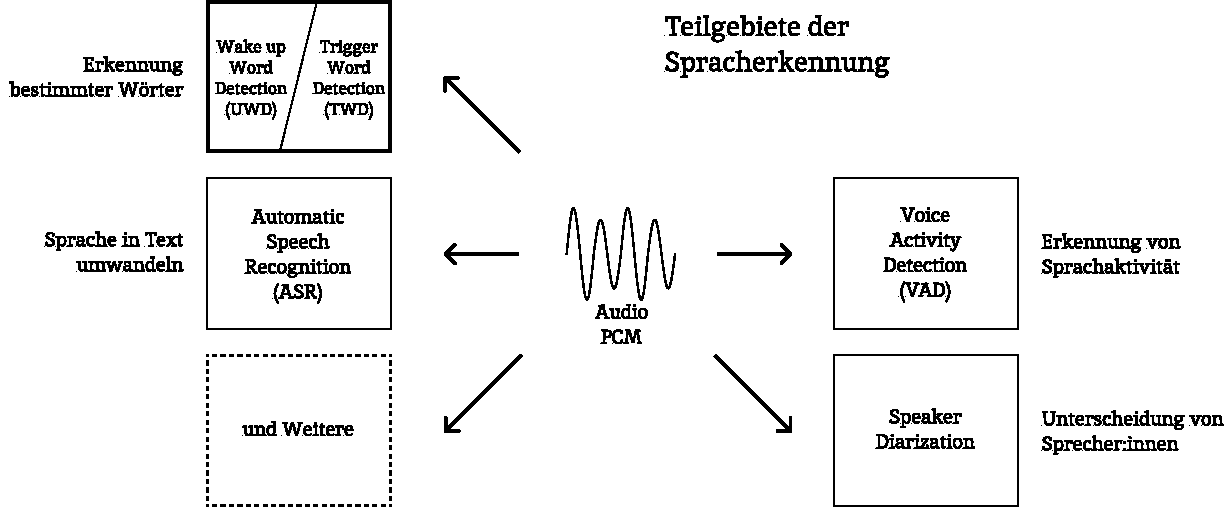
\includegraphics[width=1.0\linewidth]{img/asr_twd.pdf}
	\caption{Teilgebiete der Spracherkennung}
	\label{fig:asr_twd}

\end{figure}

\subsection{Fragestellung}
Wie kann eine integrierte Sprachsteuerung für eine Mobile App entwickelt werden, welche
das Erkennen von Triggerwörtern ermöglicht und wie kann diese Sprachsteuerung in eine
Mobile App integriert werden?


\subsection{Vision}
Als Vision dieser Arbeit soll eine Grundlage geschaffen werden, um ein Triggerwort
oder eine Sequenz von Triggerwörtern in der akustischen Sprache erkennen zu können.
Dabei sollen Methoden und Werkzeuge aus dem Bereich des Machine Learning verwendet werden.
Zudem sollen die gewonnenen Erkenntnise in eine mobile Plattform wie iOS oder Android integriert
werden. Für den Rahmen dieser Arbeit genügt die Integration in eine der genannten Plattformen.
Weiterhin soll auch das Thema Datenschutz und die ethischen Aspekte zu berücksichtigen werden.

\subsection{Ziele}
Die Ziele dieser Arbeit sind als SMART-Ziele definiert. Die Tabelle \ref{tab:smart_goals} zeigt 
die SMART-Ziele der Bachelorarbeit.

\begin{table}[h]
	\centering
	\resizebox{\textwidth}{!}{%
	\begin{tabular}{|l|p{12cm}|}
	\hline
	\textbf{Ziel} & \textbf{SMART-Kriterien} \\ \hline
	Erkennen von Triggerwörtern & \textbf{Spezifisch:} Entwicklung eines Modells zur Erkennung von 
								 von einem oder mehreren Triggerwörtern in der akustischen Sprache. 
								 \textbf{Messbar:} Erfolgsrate der korrekten Erkennung.
								 \textbf{Ausführbar:} Umsetzung mit aktuellen Machine 
								 Learning-Methoden. 
								 \textbf{Realistisch:} Realisierbar mit bestehenden Technologien. 
								 \textbf{Terminiert:} Fertigstellung bis zum Ende der 
								 Bachelorarbeit. \\ \hline
	Integration in eine Mobile App & \textbf{Spezifisch:} Einbindung des erarbeiteten Modells in 
									 eine iOS- oder Android-App. 
									 \textbf{Messbar:} Durch User-Tests und Messung der Erfolgsrate
									 \textbf{Ausführbar:} Machbar mit vorhandenen 
									 Entwicklungswerkzeugen und Plattformen. 
									 \textbf{Realistisch:} Durchführbar innerhalb des 
									 Projektzeitrahmens. 
									 \textbf{Terminiert:} Integration bis zum Abschluss der 
									 Bachelorarbeit. \\ \hline
	Datenschutz und Ethik & \textbf{Spezifisch:} Gewährleistung von Datenschutz und ethischer 
							Konformität bei der Erstellung des Datensatzes. 
							\textbf{Messbar:} Erfüllung spezifischer Datenschutzrichtlinien und 
							ethischer Standards im Datenerhebungsprozess. 
							\textbf{Ausführbar:} Einhaltung von Best Practices und Richtlinien 
							während der Datensammlung und -aufbereitung. 
							\textbf{Realistisch:} Umsetzbar durch sorgfältige Planung und 
							Überprüfung der Prozesse. 
							\textbf{Terminiert:} Kontinuierliche Überwachung und Anpassung 
							während der Datensatzerstellung.\\ \hline
									 
									 
	\end{tabular}}
	\caption{SMART Ziele der Bachelorarbeit}
	\label{tab:smart_goals}
\end{table}
	


\subsection{Abgrenzung}
Diese Arbeit befasst sich mit der Erkennung von Triggerwörtern in der akustischen Sprache. Es ist 
kein Ziel dieser Arbeit, einen vollständigen Sprachassistenten zu entwickeln. Das würde den Rahmen
dieser Arbeit sprengen. Die Resultate dieser Arbeit sollen als Grundlage für eine vollständige
Implementierung eines Sprachassistenten dienen.

\subsection{Rechtfertigung}
Apple sowie Google stellen mit Siri und Google Assistant bereits Sprachassistenten zur 
Verfügung, um Apps zu öffnen oder auch direkte Befehle auszuführen. Daher stellt sich die Frage, 
warum überhaupt eine eigene In App Sprachsteuerung? Wenn ein Sprachassistent wie Siri bereits 
API's anbieten. Als Beispiel hat Spotify eine Integration mit Siri. Es können Befehle wie 
``Hey Siri, play music on Spotify'' verwendet werden. Die Integration einer eigens entwickelten 
Sprachsteuerung in Apps ist trotz verfügbarer Lösungen wie Siri und Google Assistant aus mehreren 
Gründen vorteilhaft:


\begin{itemize}[itemsep=0pt, parsep=0pt]
    \item \textbf{Personalisierung:} Sie ermöglicht eine massgeschneiderte Nutzererfahrung, die 
	exakt auf die App und ihre Nutzer zugeschnitten ist.
    \item \textbf{Unabhängigkeit:} Apps bleiben unabhängig von den Schnittstellen und 
	Einschränkungen externer Assistenten.
    \item \textbf{Funktionalität:} Es können spezifische Funktionen implementiert werden, die über 
	das hinausgehen, was standardisierte Assistenten bieten.
    \item \textbf{Datenschutz:} Durch lokale Verarbeitung von Sprachdaten wird die Privatsphäre der 
	Nutzer besser gewahrt.
    \item \textbf{Markenidentität:} Eine einzigartige Sprachsteuerung verstärkt das Markenbild und 
	bietet ein differenziertes Nutzererlebnis.
\end{itemize}

\noindent 

\newpage \section{Grundlagen}\label{sec:grundlagen}
In diesem Kapitel werden die Grundlagen für die Arbeit erläutert. Dabei wird auf die Themen
Audioverarbeitung und Machine Learning eingegangen.

\subsection{Audio}
In der digitalen Welt werden Schallwellen, die durch eine Reihe von numerischen Werten
repräsentiert. (\cite[p.9]{somberg2019audioapi}) beschreibt Audio als: \glqq Fundamentally,
audio can be modeled as waves in an elastic medium. In our normal everyday experience, the elastic
medium is air, and the waves are air pressure waves.\grqq \ Audiosignale werden durch die Funktion
\(A(t)\) repräsentiert, wobei \(t\) die Zeit und \(A(t)\) die Amplitude zum
Zeitpunkt \(t\) angibt. Die Amplitude ist die Stärke des Signals und die Zeit repräsentiert die
Position des Signals. Grundsätzlich ist Audio ein kontinuierliches Signal, in der digitalen Welt 
können jedoch nur diskrete Werte dargestellt werden. Das kontinuierliche Signal muss somit in 
diskrete Werte umgewandelt werden. Dieser Vorgang wird als \textit{Sampling} bezeichnet 
(\cite[Chapter~3.1]{tarr2018hackaudio}). 


\subsubsection{Sampling}
Ein früher Ansatz zur digitalen Darstellung von analogen Signalen war die Pulse-Code-Modulation
(PCM). Dieses Verfahren wurde bereits in den 1930er Jahren von Alec H. Reeves, parallel zum 
Aufkommen der digitalen Telekommunikation, entwickelt (\cite[p.~57]{deloraine1965pcm}). Im Grundsatz 
wird es heute noch in modernen Computersystemen nach dem gleichen Verfahren angewendet.

\noindent \newline
Es folgt eine Definition von Sampling. Ein kontinuierliches Signal \(A(t)\)
wird in bestimmten Zeitintervallen \(T_s\) gesampelt. Diese Zeitintervalle werden auch als
Sampling-Periode bezeichnet. Die Sampling-Rate \(F_s = \displaystyle\frac{1}{T_s}\) gibt die Anzahl
der Samples pro Sekunde an. Angenommen wir haben ein Signal mit einer Sampling-Periode
von \(T_s = 0.001\). Um nun die Sampling-Rate zu berechnen, müssen wir den Kehrwert der
Sampling-Periode berechnen. \(F_s = \displaystyle\frac{1}{0.001} = 1000\). Somit erhalten wir eine
Sampling-Rate von \(1000\) Samples pro Sekunde. Typische Sampling-Raten sind \(44100\) Hz
oder \(48000\) Hz. Ein Hertz entspricht einer Frequenz von einem Sample pro Sekunde. 
Ein weiter wichtiger Begriff ist die \textit{Nyquist-Frequenz}. Die Nyquist-Frequenz \(F_n\) ist 
die Hälfte der Sampling-Rate \(F_n = \displaystyle\frac{F_s}{2}\) und muss mindestens doppelt so 
hoch sein wie die höchste Frequenz des Signals. Ist diese Eigenschaft erfüllt, kann das 
Signal ohne Informationsverlust rekonstruiert werden (\cite[Chapter~3.1]{tarr2018hackaudio}). 
Mehr dazu folgt im Unterkapitel \textit{Fourier-Analyse}.

\noindent \newline
Weiter ist es wichtig zu verstehen, dass ein Sample ein diskreter Wert ist und in digitalen 
Systemen durch eine bestimmte Anzahl von Bits dargestellt wird. Die Anzahl der Bits wird
als \textit{Bit-Depth} bezeichnet und bestimmt die Auflösung des Signals. Typische
Bit-Depth Werte sind \(16\) oder \(24\) Bit (\cite[p.10]{somberg2019audioapi}).

\subsubsection{Frames, Channels, Buffers}
Ebendfalls wichtig ist das Verständnis von Frames, Channels und Buffers. Da diese Arbeit sich mit
Audio-Systemen beschäftigt, ist es wichtig, die Begriffe \textit{Frame}, \textit{Channel} und
\textit{Buffer} zu verstehen. Fangen wir mit dem Begriff \textit{Channel} an. Ein Channel kann als
ein einzelnes Audio-Signal verstanden werden. Ein Mono-Signal hat genau nur einen Channel. Ein
Stereo-Signal hat zwei Channels. Ein Surround-Signal hat mehr als zwei Channels. usw.
Nun zum Begriff \textit{Frame}. Ein Frame entspricht einem Sample pro Channel. Weiter sind Frames
in Buffers organisiert. Ein Buffer ist eine Sammlung von Frames. Typischerweise werden Buffers in
Grössen von \(64\), \(128\), \(256\), \(512\) oder \(1024\) Frames organisiert. Die Abbildung
\ref{fig:frames_channels_buffers} zeigt die Beziehung zwischen Frames, Channels und Buffers.
Die Abbildung wurde basierend auf (\cite[p.10]{somberg2019audioapi}) erstellt und verdeutlicht die
Beziehung zwischen Frames, Channels und Buffers.

\begin{figure}[h]
	\centering
	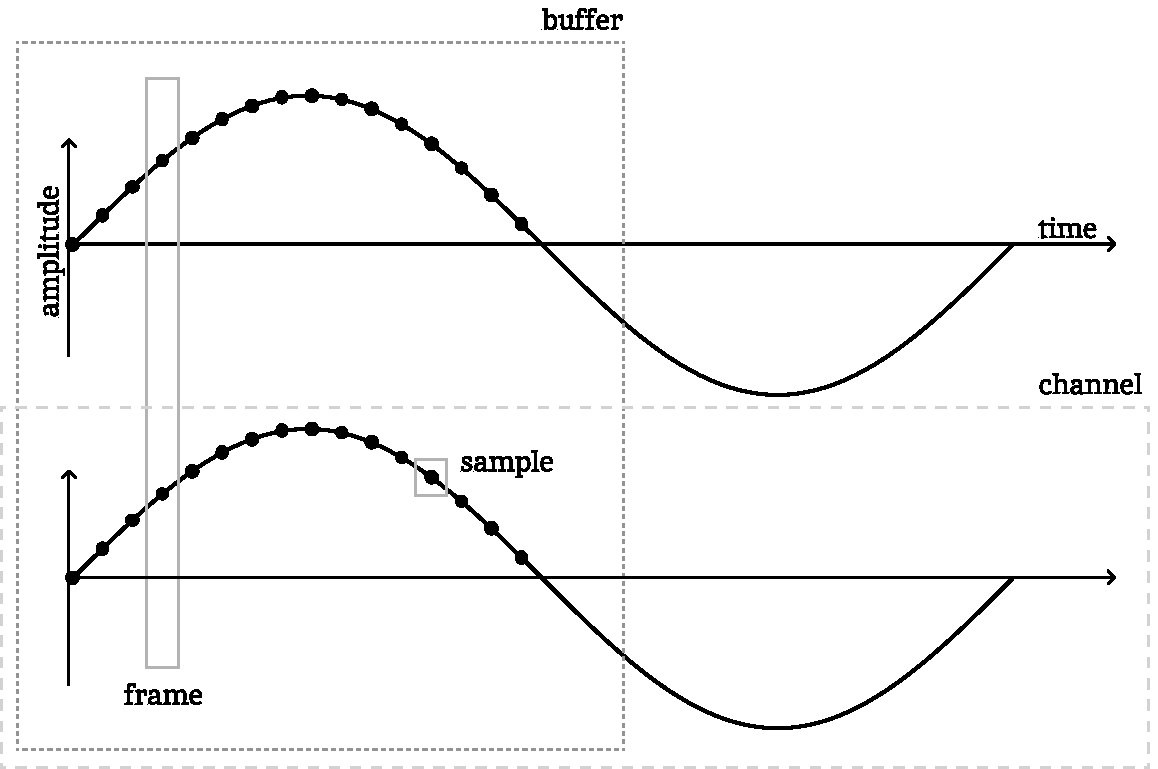
\includegraphics[width=0.7\linewidth]{img/audio-nutshell.pdf}
	\caption{Frames, Channels und Buffers}
	\label{fig:frames_channels_buffers}
\end{figure}

\subsubsection{Buffers im Detail}
Ein Buffer im Kontext von Audio ist eine aufeinanderfolgende Sammlung von Frames. Die bereits
angesprochene Grösse eines Buffers bestimmt im wesentlichen die Latenzzeit des Systems. Kleine
Buffer-Grössen haben eine geringe Latenzzeit, während grosse Buffer-Grössen eine hohe Latenzzeit
haben (\cite[p.10]{somberg2019audioapi}). Der Trade-Off ist dass kleine Buffer-Grössen
zu einer höheren CPU-Auslastung führen, während bei grossen Buffer-Grössen das nicht der Fall ist.
Das liegt daran, dass bei kleinen Buffer-Grössen die CPU häufiger aufgerufen wird, um die Buffers
zu verarbeiten.

\noindent \newline
Nun betrachten wir die mögliche Anordnung eines Buffers, wie in der folgenden Tablle 
\ref{tab:frames_buffers} dargestellt. Es gibt zwei Möglichkeiten, wie Buffers angeordnet werden
können: \textit{Interleaved} und \textit{Non-Interleaved}. Bei der \textit{Interleaved}-Anordnung
werden die Samples der einzelnen Channels nacheinander in sequentieller Reihenfolge in den Buffer
geschrieben. Im Gegensatz dazu werden bei der \textit{Non-Interleaved}-Variante die Samples
eines Channels nacheinander in den Buffer geschrieben, bevor die Samples des nächsten Channels
hinzugefügt werden. Dieser Vorgang wird für jeden Channel wiederholt. Die Tabelle
\ref{tab:frames_buffers} zeigt die Unterschiede zwischen den beiden Anordnungen. Jede Zelle der
Tabelle entspricht einem Sample. L und R stehen exemplarisch für die Channels Left und Right.
Die erste Zeile entspricht der \textit{Interleaved}-Anordnung und die zweite Zeile der
\textit{Non-Interleaved}-Anordnung. Die Abbildung wurde basierend auf
(\cite[p.11]{somberg2019audioapi}) erstellt.

\begin{table}[h]
	\centering
	\begin{tabularx}{\textwidth}{|X|X|X|X|X|X|X|X|}
		\hline
		L & R & L & R & L & R & L & R \\
		\hline
		L & L & L & L & R & R & R & R \\
		\hline
	\end{tabularx}
	\caption{Frames in Interleaved und Non-interleaved Buffers}
	\label{tab:frames_buffers}
\end{table}

\noindent
Mit diesem Wissen kennen wir nun die Unterschiede zwischen den beiden Anordnungen. Für die
Anwendung ist es wichtig zu verstehen, mit welcher Anordnung die verwendete API arbeitet.

\subsection{Audio APIs}
Audio APIs sind im Bereich der Audioverarbeitung von essentieller Bedeutung. Sie bieten eine
Schnittstelle, welche den Zugriff auf vielfältige Audiofunktionen erlaubt. Ohne solche APIs müssten
Entwickler die Audioverarbeitung von Grund auf neu implementieren.

\noindent \newline
In der Erarbeitungsphase dieser Arbeit kristallisierten sich zwei primäre Anwendungsgebiete heraus.
Erstens die intensive Auseinandersetzung mit Audioverarbeitung in Python, um tieferes Verständnis
für die Materie zu entwickeln. Zweitens die Notwendigkeit, eine Audio API in eine mobile
Applikation zu integrieren. Im Kontext dieser Arbeit werden sie als \textit{Audio API für Analyse}
und \textit{Audio API für Integration} bezeichnet.

\noindent \newline
Im Bereich der \textit{Analyse} fiel die Wahl auf folgende APIs:

\begin{itemize}[itemsep=0pt, parsep=0pt]
	\item \textbf{PyAudio:} Eine verbreitete Schnittstelle in Python zur Audioverarbeitung.
	\item \textbf{SoundDevice:} Eine vielseitige Python-Bibliothek für Audioverarbeitungsaufgaben.
	\item \textbf{librosa:} Eine Bibliothek, die speziell auf die Analyse von Audiosignalen
	      ausgerichtet ist.
\end{itemize}

\noindent
Im Kontext der \textit{Integration} standen folgende APIs im Fokus:

\begin{itemize}[itemsep=0pt, parsep=0pt]
	\item \textbf{AVAudioEngine:} Eine leistungsfähige Schnittstelle primär für die Plattformen iOS
	      und macOS.
	\item \textbf{AudioTrack:} Eine spezialisierte API für Audioanwendungen auf Android-Geräten.
\end{itemize}

\noindent
Die folgenden Abschnitte werden tiefer auf jeweils eine API pro Anwendungsgebiet eingehen. 
Insbesondere wird auf die Echtzeitverarbeitung von Audiodaten eingegangen und Beispiele dazu
gezeigt.

\subsubsection{Audio API für Analyse}
Python zeichnet sich durch eine beeindruckende Auswahl an Bibliotheken für datenanalytische Aufgaben
aus, zu denen auch NumPy, SciPy, Pandas und Matplotlib gehören. In dieser Arbeit wurde zunächst
\textbf{PyAudio} in Erwägung gezogen. PyAudio ist als Schnittstelle zur PortAudio-Bibliothek
bekannt, die plattformübergreifende Audioverarbeitungsfunktionen bereitstellt. Trotz ihrer
intuitiven Funktionen für Aufnahme und Wiedergabe wurde PyAudio letztlich aufgrund von
Inkompatibilitäten mit der gewählten Entwicklungsumgebung verworfen.


\noindent \newline
In dieser Arbeit wurde \textbf{SoundDevice} als Alternative zu PyAudio verwendet. Daher wird eine 
kurze Implementierung von SoundDevice gezeigt, welches das kontinuierliche Streamen von Audio in
Chunks ermöglicht. Der folgende Source Code (\ref{lst:sounddevice}) zeigt die Implementierung.

\begin{lstlisting}[caption={SoundDevice Audio Stream}, label={lst:sounddevice}]
import sounddevice as sd

def stream_audio(chunk_duration, samplerate=16000):
    """Stream audio in chunks."""
    with sd.InputStream(samplerate=samplerate, channels=1) as stream:
        while True:
            audio_chunk, _ = stream.read(int(samplerate * chunk_duration))
            yield audio_chunk
\end{lstlisting}

\noindent
Mit praktisch fünf Zeilen Code kann ein Audio-Stream in Chunks mit einer bestimmten Dauer
erzeugt werden. Diese Einfachheit und Abstraktion ist ein grosser Vorteil von SoundDevice. Wie wir 
sehen werden, wird die Implementierung mit der \textbf{AVAudioEngine} API für iOS und macOS nicht
so einfach sein.


\newpage
\subsubsection{Audio API für Integration} \label{sec:audio_api_integration}
Dieser Abschnitt befasst sich mit dem Thema Audio API für Integration in eine iOS App. Die Wahl 
fiel auf die \textbf{AVAudioEngine} API für iOS und macOS. Im der folgenden Abbildung 
\ref{fig:avaudioengine} wird gezeigt, wie ein kontinuierlicher Audio-Stream mit AVAudioEngine 
aufgenommen werden kann.

\begin{figure}[h]
	\centering
	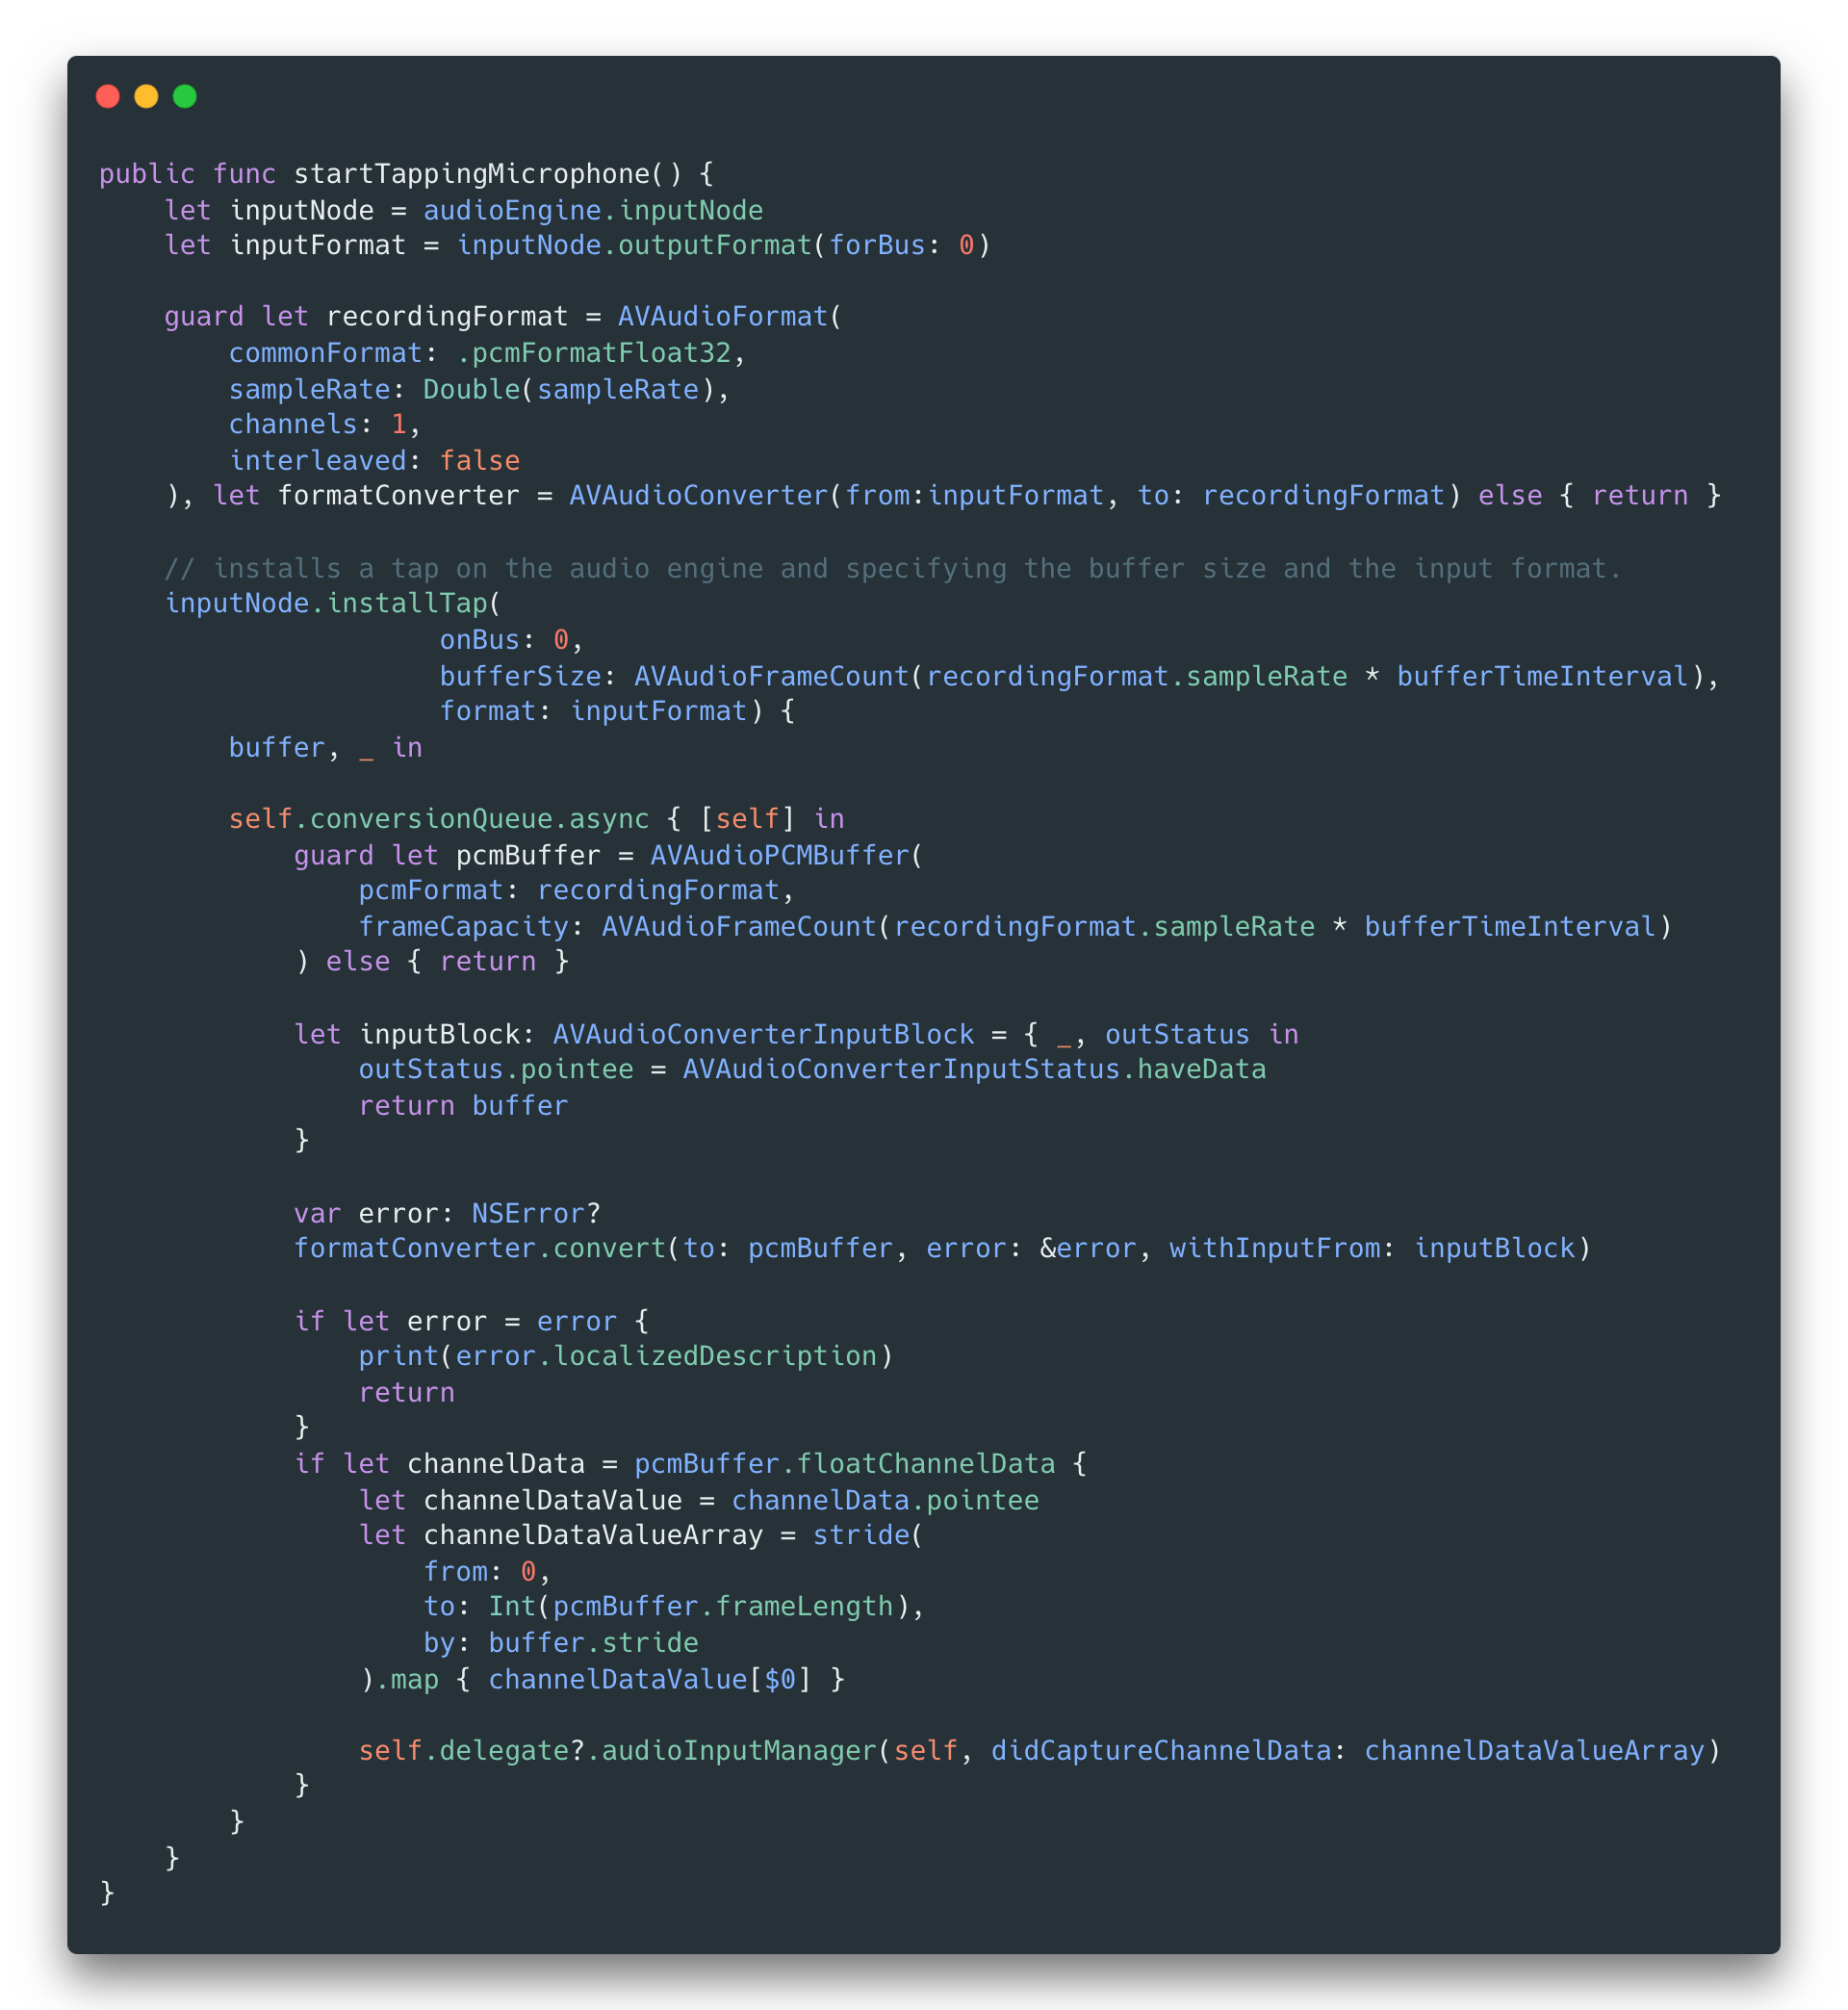
\includegraphics[width=1.0\linewidth]{img/avaudioengine.png}
	\caption{AVAudioEngine}
	\label{fig:avaudioengine}
\end{figure}


\noindent \newline
Im Gegensatz zu SoundDevice ist die Implementierung mit AVAudioEngine nicht so abstrakt. Man muss
einige Konzepte verstehen, um die API effektiv nutzen zu können. Beispielsweise wird in diesem Code
eine Konvertierung der Samplerate von \(48000\) Hz auf \(16000\) Hz durchgeführt. Ebenfalls müssen 
die Buffer-Grösse, Bit-Depth, Channels und die Anordnung der Frames definiert werden.

\newpage \subsection{Fourier-Analyse}
Die Fourier-Analyse befasst sich mit der Zerlegung von Funktionen in Frequenzkomponenten. Die
Fourier-Analyse ist ein wichtiges Konzept in der Signalverarbeitung und findet breite Anwendung
in der Audioverarbeitung. Daher ist ein Grundverständnis für diese Arbeit relevant.

\subsubsection{Fourier-Transformation}
Die Fourier-Transformation ist ein zentrales Werkzeug der Fourier-Analyse. Sie ermöglicht die
Zerlegung von Funktionen in ihre Frequenzkomponenten und die Rekonstruktion von Funktionen aus
diesen Komponenten. Dies wird als Fourier-Analyse und Fourier-Synthese bezeichnet. Dieses Konzept
wird auch von Prof. Dr. Weitz in seinem Video zu Fourier-Analyse erläutert
(\cite[2:20]{weitz2023fourier}). Mathematisch ausgedrückt wird die kontinuierliche
Fourier-Transformation eines Signals \( f(t) \) wie folgt definiert
(\cite[Chapter~5]{hansen2014fourier}):

\begin{equation*}
	F(\omega) = \int_{-\infty}^{\infty} f(t) e^{-i \omega t} \, dt
	\label{eq:fourier_transform}
\end{equation*}

\noindent
\(F(\omega)\) ist die Fourier-Transformation von \(f(t)\)
(\cite[49:27]{weitz2023fourier}). Als kleines Rechenbeispiel betrachten wir die
Fourier-Transformation der Rechteckfunktion \( \text{rect}(x) \), die wie folgt definiert ist:

\[
	\text{rect}(x) =
	\begin{cases}
		1 & \text{für } -1 \leq x \leq 1 \\
		0 & \text{sonst}
	\end{cases}
\]

\noindent
Die Fourier-Transformation der Funktion \( \text{rect}(x) \) kann wie folgt berechnet werden:

\begin{equation*}
	\begin{split}
		F(\omega) &= \int_{-\infty}^{\infty} \text{rect}(x) e^{-i \omega x} \, dx \\
		&= \int_{-1}^{1} e^{-i \omega x} \, dx \\
		&= \frac{1}{-i \omega} \left[ e^{-i \omega x} \right]_{-1}^{1} \\
		&= \frac{1}{-i \omega} \left( e^{-i \omega} - e^{i \omega} \right) \\
		&= \frac{1}{-i \omega} \left( \cos(\omega) - i \sin(\omega) - \cos(\omega) - i \sin(\omega) \right) \\
		&= \frac{1}{-i \omega} \left( -2 i \sin(\omega) \right) \\
		&= \frac{2 \sin(\omega)}{\omega}
	\end{split}
\end{equation*}
\noindent

\noindent
\newline
Somit ist die Fourier-Transformation der Rechteckfunktion \( \text{rect}(x) \) gleich
\( \displaystyle\frac{2 \sin(\omega)}{\omega} \).

\begin{figure}[h]
	\centering
	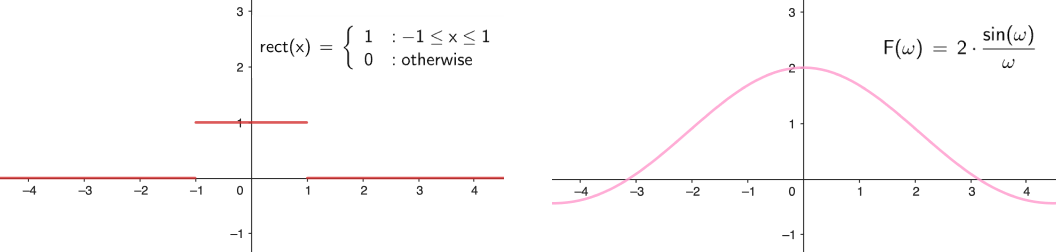
\includegraphics[width=0.8\linewidth]{img/example-fourier-trans.png}
	\caption{Rechteckfunktion und ihre Fourier-Transformation}
	\label{fig:fourier_transform}
\end{figure}

\noindent
Die Abbildung \ref{fig:fourier_transform} stellt die \( \text{rect}(x) \) Funktion und ihre
Fourier-Transformation, die als \( \text{sinc}(\omega) \) bezeichnet wird, dar. Die Nullstellen
\( \pm \pi, \pm 2 \pi, \pm 3 \pi, \dots \) der \( \text{sinc}(\omega) \) Funktion deuten darauf
hin, dass die \( \text{rect}(x) \) Funktion bei diesen Frequenzen keine Energie besitzt. Die
primäre Energie der Funktion liegt bei \( \omega=0 \). Beispiel adaptiert von
(\cite[Chapter~5 - Example~5.1]{hansen2014fourier}).


\subsubsection{Diskrete Fourier-Transformation}

Die diskrete Fourier-Transformation (DFT) stellt eine diskrete Variante der kontinuierlichen
Fourier-Transformation dar und wird speziell auf diskrete Signale angewendet. In digitalen
Systemen sind Signale typischerweise diskret und bestehen aus einzelnen Samples, weshalb die DFT
besonders relevant für solche Anwendungen ist. Die mathematische Definition der DFT ist
(\cite[Chapter~3]{hansen2014fourier}):

\[
	F(k) = \sum_{n=0}^{N-1} f(n) \cdot e^{-\frac{2\pi i}{N} kn}
\]

\noindent \newline
Zur Veranschaulichung betrachten wir ein Source Code Beispiel (\ref{lst:dft_example}). 
Wir haben eine Funktion \(f(t)\) und unterteilen diese in \(N\) Samples. Die DFT berechnet nun die 
Frequenzkomponenten des Signals. Die Abbildung \ref{fig:dft_example} zeigt ein Beispiel für ein 
Signal \(f(t)\) mit \(N=5\) Samples.

\[ f(t) = 1.5 \cos(t) + 0.25 \sin(t) + 2 \sin(2t) + \sin(3t) \].

\begin{lstlisting} [caption={Unterteilung der Funktion \(f(t)\) in 5 Samples}, label={lst:dft_example}]
import numpy as np
import matplotlib.pyplot as plt

def f(x):
    return 1.5 * np.cos(x) + 0.25 * np.sin(x) + 2 * np.sin(2*x) + np.sin(3*x)

N_SAMPLES = 5

x_curve = np.linspace(0, 2*np.pi, 100) # 100 Punkte zwischen 0 und 2pi
x_points = np.linspace(0, 2*np.pi, N_SAMPLES) # 5 Punkte zwischen 0 und 2pi

plt.plot(x_curve, f(x_curve))
plt.plot(x_points, f(x_points), 'o') # Plotte die 5 Punkte
\end{lstlisting}

\begin{figure}[h]
	\centering
	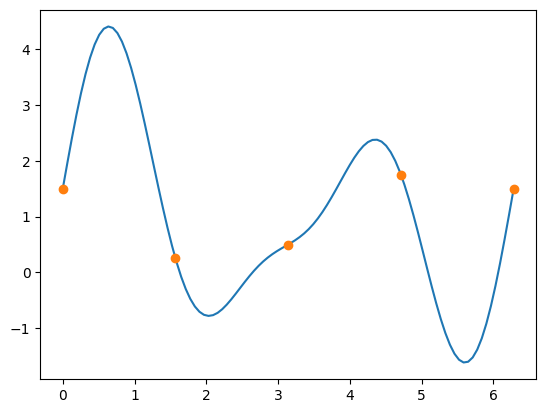
\includegraphics[width=0.60\linewidth]{img/dft.png}
	\caption{Funktion \( f(x) \) mit 5 Samples}
	\label{fig:dft_example}
\end{figure}

\noindent
Nun berechnen wir die DFT der 5 Samples. Dazu verwenden wir die \texttt{fft} Funktion aus der
\texttt{numpy} Bibliothek. Das Resultat ist ein Array mit \(N\) komplexen Zahlen. Die Tabelle
\ref{tab:dft_example_table} zeigt die Funktion \(f(x)\) und die DFT der 5 Samples.

\begin{lstlisting}
fhat = np.fft.fft(f(x_points), N_SAMPLES)
\end{lstlisting}

\begin{table}[h]
	\centering
	\begin{tabular}{|c|c|c|c|c|c|}
		\hline
		         & 0                & 1                & 2                & 3                & 4                \\
		\hline
		\(f(x)\) & 1.5              & 0.25             & 0.5              & 1.75             & 1.5              \\
		\hline
		dft      & \(5.50 + 0.00i\) & \(0.22 + 1.92i\) & \(0.78 - 0.45i\) & \(0.78 + 0.45i\) & \(0.22 - 1.92i\) \\
		\hline
	\end{tabular}
	\caption{\(f(x)\) und die DFT der 5 Samples}
	\label{tab:dft_example_table}
\end{table}

\noindent
Mit den Frequenzkomponenten der DFT können Signale manipuliert werden, etwa durch Filtern
bestimmter Frequenzbereiche. Um das ursprüngliche Signal wiederzuerlangen, wenden wir die inverse
DFT an. Die Formel der inversen DFT, welche das Signal rekonstruiert, lautet
(\cite[Chapter~3]{hansen2014fourier}):


\[
	f(n) = \frac{1}{N} \sum_{k=0}^{N-1} F(k) \cdot e^{\frac{2\pi i}{N} kn}
\]

\begin{lstlisting}
reconstructed_manual = np.zeros_like(x_points, dtype=np.complex128)

dt = x_points[1] - x_points[0] # Abstand zwischen zwei Punkten
T = N_SAMPLES * dt # Periode des Signals

for n in range(N_SAMPLES):
    # Rekonstruiert Signal mit Fourier-Koeffizienten, neg. Freq. bei n > N_SAMPLES/2.
    freq = n / (2*np.pi) if n <= N_SAMPLES//2 else (n - N_SAMPLES) / (2*np.pi)
    reconstructed_manual += fhat[n] * np.exp(1j * 2 * np.pi * freq * x)

reconstructed_manual = (reconstructed_manual / N_SAMPLES).real
reconstructed = np.fft.ifft(fhat).real # Rekonstruiertes Signal mit ifft
\end{lstlisting}

\begin{figure}[h]
	\centering
	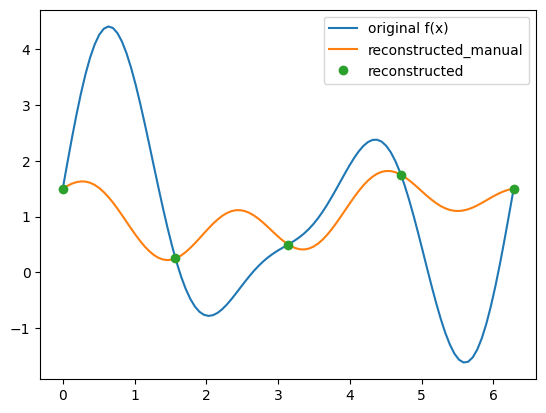
\includegraphics[width=0.60\linewidth]{img/dft_reconstructed.png}
	\caption{Rekonstruktion des Signals \(f(x)\)}
	\label{fig:dft_example_reconstructed}
\end{figure}

\noindent
\newline
Die Abbildung \ref{fig:dft_example_reconstructed} zeigt die ursprüngliche Funktion \(f(x)\) und die
rekonstruierte Funktionen \texttt{reconstructed (n=5)} und \texttt{reconstructed (n=nyquist)}.
Die Annäherung der mit der inversen DFT rekonstruierten Funktion an die ursprüngliche Funktion ist
bei \(n=5\) deutlich sichtbar. Bei \(n=nyquist\) ist die Annäherung nahezu perfekt, wenn nicht sogar
perfekt. Die Sampling-Rate bei der Nyquist angenäherten Funktion ist das Doppelte der höchsten
Frequenz des Signals. Das ist in diesem Fall \(2 \cdot 3 + 1 = 7\).

\subsubsection{Aliasing}
Aliasing tritt auf, wenn ein Signal bei einer nicht ausreichend hohen Samplingrate digital erfasst
wird, wodurch Frequenzen des Signals fehlinterpretiert werden können. Als allgemeines Beispiel wenn
ein Sinussignal mit einer Frequenz von 1200 Hz betrachtet wird und dieses mit einer Samplingrate
von nur 1000 Hz aufgenommen wurde, könnte das digitalisierte Signal so aussehen, als ob das
ursprüngliche Signal eine Frequenz von 200 Hz hätte. Das ist, als ob man ein sich schnell
drehendes Rad filmt und auf dem Video wirkt es, als würde es sich langsamer oder sogar rückwärts
drehen. Um solche Fehler zu verhindern, sollte die Samplingrate stets mindestens das
Doppelte der höchsten Frequenz des Signals betragen, ein Grundsatz, der als Nyquist-Kriterium
bekannt ist. (\cite[]{weitz2023fourier}).

\subsection{Spektrogramm}
Mit einem Verständnis der Grundlagen der Fourier-Analyse können wir die Bedeutung des Spektrogramms
erfassen. Ein Spektrogramm bietet eine visuelle Darstellung der verschiedenen Frequenzen, die in
einem Signal über die Zeit hinweg vorhanden sind. Ein Spektrogramm wird wie folgt definiert:

\begin{displayquote}
	''A spectrogram is a three-dimensional visualization of a signal’s amplitude over frequency and
	time. Many audio signals are comprised of multiple frequencies occurring simultaneously, with
	these frequencies often changing over time.'' (\cite[Chapter~15.2.1]{tarr2018hackaudio})
\end{displayquote}

\noindent
Im Bereich des Machine Learning, insbesondere bei der Spracherkennung, nimmt das Spektrogramm eine
zentrale Position ein. Die Fourier-Transformation eines Audiosignals in seine Frequenzkomponenten
resultiert in einem Verlust der zeitlichen Informationen durch die Anwendung der FFT. Für Aufgaben
wie die Spracherkennung ist es jedoch von grundlegender Bedeutung, nicht nur die im Signal
vorhandenen Frequenzen zu identifizieren, sondern auch den Zeitpunkt ihres Auftretens zu bestimmen.
Hier schafft das Spektrogramm Abhilfe, da es die zeitliche Abfolge der Frequenzen sichtbar macht.
Diese Fähigkeit ist insbesondere für das Erkennen der Sequenz gesprochener Wörter in einem Satz von
Bedeutung (\cite{chaudhary2020}). Somit verknüpft das Spektrogramm zeitliche und frequenzbezogene
Informationen, was es zu einem wichtigen Instrument für die Spracherkennung und andere Machine
Learning-Anwendungen macht. Abbildung \ref{fig:spectrogram} zeigt ein Beispiel eines Spektrogramms,
das im Rahmen dieser Arbeit entwickelt wurde. Das Spektrogramm wurde unter Verwendung der
Python-Bibliotheken \texttt{PyQt6} für die Echtzeit-Visualisierung und \texttt{soundevice} für den
Zugriff auf die Audio-Hardware generiert.

\begin{figure}[h]
	\centering
	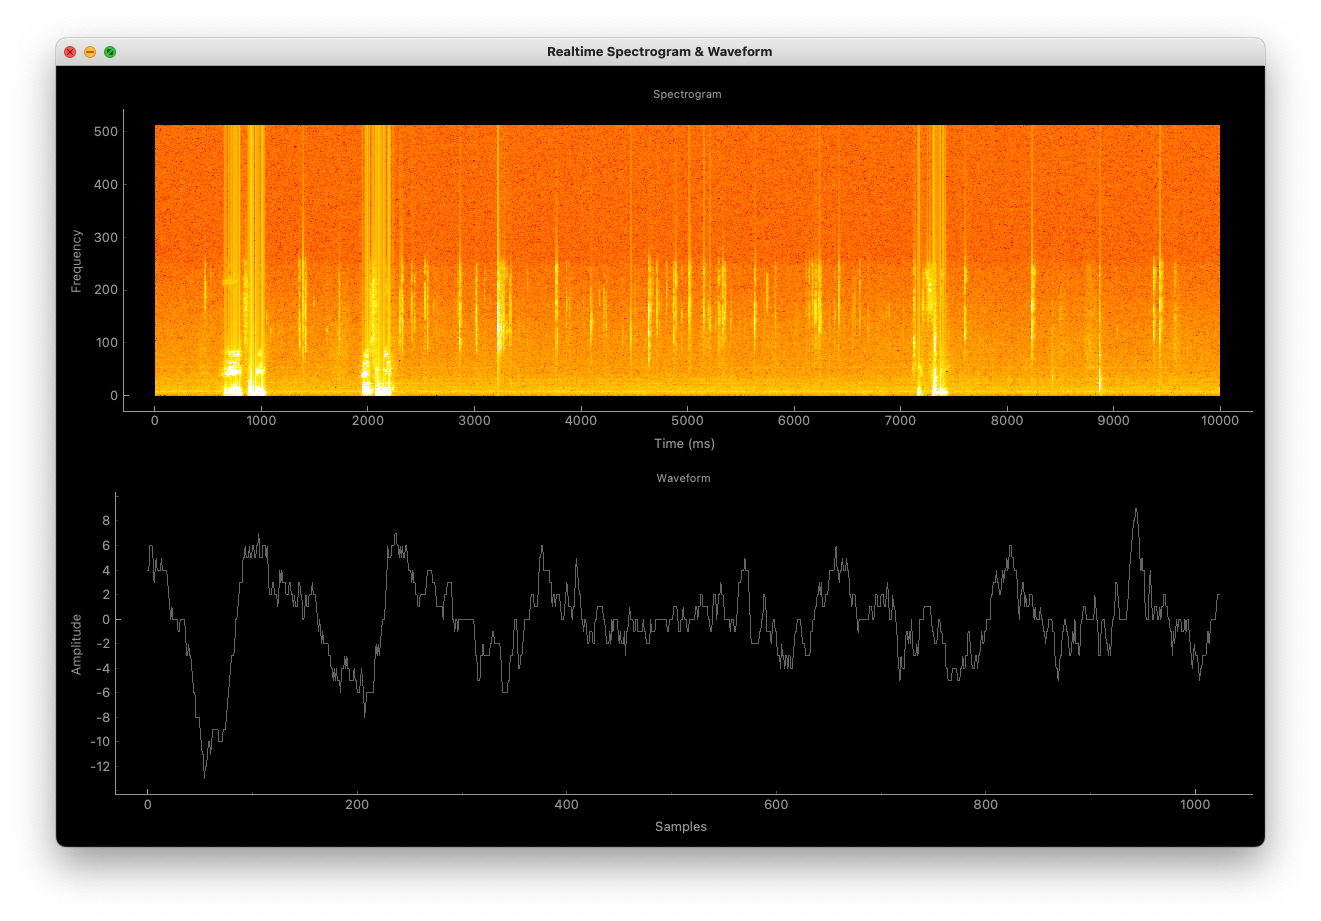
\includegraphics[width=0.73\linewidth]{img/spectrogram.png}
	\caption{Spektrogramm}
	\label{fig:spectrogram}
\end{figure}

\subsection{Machine Learning}
Dieses Kapitel erläutert die grundlegenden Konzepte von Machine Learning, die für die
Spracherkennung relevant sind. Es fokussiert sich auf Deep Neural Networks (DNN), Convolutional
Neural Networks (CNN) und Recurrent Neural Networks (RNN). Um ein detailiertes Verständnis von
neuronalen Netzen zu erhalten, empfiehlt sich die Lektüre von (\cite{weidman2019deep}).

\subsubsection{Neuronale Netze}
Unter Neuronalen Netzen versteht man im Allgemeinen eine Reihe von Berechnungen, die von der
Funktionsweise des menschlichen Gehirns inspiriert sind. Im Grunde sind es mathematische Modelle,
die aus einer Reihe von miteinander verbundenen Nodes bestehen, die als Neuronen bezeichnet werden.
Im einfachsten Fall bestehen Neuronen aus Inputs \(x_{1}, x_{2}, \dots, x_{n}\), Gewichten
\(w_{1}, w_{2}, \dots, w_{n}\), einem Bias \(b\) einer Aktivierungsfunktion \(f\) und einem Output
\(y\). Die Abbildung \ref{fig:neuron} zeigt ein einfaches Beispiel eines Neurons.

\begin{figure}[h]
	\centering
	\begin{tikzpicture}
		% Nodes for x1, x2
		\foreach \i/\y in {1/-1,2/-2} {
				\node[circle,fill=gray!30,minimum size=1cm] (x\i) at (0,\y) {$x_{\i}$};
				\node (w\i) at (2,\y) {$w_{\i}$};
				\draw[->] (x\i) -- (w\i) -- (4,-2.5);
			}

		% Nodes for xn
		\node[circle,fill=gray!30,minimum size=1cm] (xn) at (0,-4) {$x_{n}$};
		\node (wn) at (2,-4) {$w_{n}$};
		\draw[->] (xn) -- (wn) -- (4,-2.5);

		% Dots
		\node at (0,-3) {$\vdots$};
		\node at (2,-3) {$\vdots$};

		% Summation and Activation
		\node[circle,draw,minimum size=2cm] (sum) at (5,-2.5) {$\Sigma | f$};
		\node (activation) at (9,-2.5) {$f\left(b+\sum_{i=1}^{n}x_{i}\cdot w_{i}\right) = y$};
		\draw[->] (sum) -- (activation);

		% Bias
		\node (b) at (3,0) {$b$};
		\draw[->] (b) -- (sum);
	\end{tikzpicture}

	\caption{Neuron eines neuronalen Netzes}
	\label{fig:neuron}

\end{figure}


\noindent
Neuronale Netze sind gut geeignet, um komplexe Probleme zu lösen, die nicht besonders einfach mit
traditionellen Algorithmen gelöst werden können. Ein Beispiel dafür ist die Spracherkennung oder
auch die Bilderkennung. Netzwerke werden trainiert, um die richtigen Gewichte
\(w_{1}, w_{2}, \dots, w_{n}\) und den Bias \(b\) zu finden, um die gewünschte Ausgabe zu erhalten.

\noindent \newline
Als nächtest betrachten wir ein kleines Beispiel eines neuronalen Netzes mit drei Layern.
Die Abbildung \ref{fig:neural_network} soll das Konzept eines neuronalen Netzes veranschaulichen.

\vspace{0.5cm}

\begin{figure}[h!]
	\centering
	\begin{tikzpicture}[
			neuron/.style={circle, draw=black, minimum size=1cm},
			layer/.style={anchor=center}
		]

		\foreach \i in {1,...,5} { % Input Layer
				\node[neuron] (I-\i) at (0, \i*1.5) {$x_{\pgfmathtruncatemacro\result{6-\i}\result}$};
			}

		\foreach \i in {1,...,3} { % Hidden Layer
				\node[neuron] (H-\i) at (3, \i*2.5 -0.5) {$h_{\pgfmathtruncatemacro\result{4-\i}\result}$};
			}

		\foreach \i in {1,...,2} { % Output Layer
				\node[neuron] (O-\i) at (6, \i*3.5 -0.5) {$y_{\pgfmathtruncatemacro\result{3-\i}\result}$};
			}

		\foreach \i in {1,...,5} % Connect Input Layer to Hidden Layer
		\foreach \j in {1,...,3} {
				\draw[->, thick] (I-\i) -- (H-\j);
			}

		\foreach \i in {1,...,3} % Connect Hidden Layer to Output Layer
		\foreach \j in {1,...,2} {
				\draw[->, thick] (H-\i) -- (O-\j);
			}

	\end{tikzpicture}
	\caption{Ein neuronales Netzwerk mit drei Layern.}
	\label{fig:neural_network}
\end{figure}


\noindent \newline \textbf{Aktivierungsfunktionen} \newline
Aktivierungsfunktionen sind ein wichtiger Bestandteil von neuronalen Netzen. Sie werden verwendet,
um die Ausgabe eines Neurons zu berechnen. Es gibt verschiedene Arten von Aktivierungsfunktionen.
Die bekanntesten sind die \textit{Sigmoid}, \textit{ReLU} und \textit{Softmax} Funktionen. Bei den 
Aktivierungsfunktionen handelt es sich um nicht-lineare Funktionen (\cite{weidman2019deep}, 
Chapter 4).


\noindent \newline \textbf{Forward Pass und Backward Pass} \newline
Zwei wichtige Konzepte in neuronalen Netzen sind der \textit{Forward Pass} und der
\textit{Backward Pass}. Der Forward Pass ist der Vorgang, bei dem die Eingabe \(x\) durch das
Netzwerk geleitet wird, um die Ausgabe \(y\) zu erhalten. Der Backward Pass ist der Vorgang, bei
dem die Gewichte \(w_{1}, w_{2}, \dots, w_{n}\) und der Bias \(b\) optimiert werden. Das Optimieren
der Gewichte und des Bias wird als \textit{Training} bezeichnet. Das geschieht, indem der Fehler 
ausgedrückt als \textit{Loss Function} minimiert wird.


\noindent \newline \textbf{Loss Function} \newline
Die Loss Function ist eine Funktion, die den Fehler zwischen der Ausgabe des neuronalen Netzes und
dem gewünschten Output misst. Die Loss Function ist ein wichtiger Bestandteil des Trainingsprozesses
eines neuronalen Netzes. Es gibt verschiedene Arten von Loss Functions. Die bekanntesten sind die
\textit{Mean Squared Error} und die \textit{Cross Entropy} Funktionen.


\subsubsection{Convolutional Neural Networks}
Convolutional Neural Networks (CNN) sind spezialisierte neuronale Netze, hauptsächlich eingesetzt 
in der Bilderkennung. Ihre Fähigkeit, komplexe Muster in Bildern zu erkennen, macht sie zu einem 
unverzichtbaren Werkzeug in der Bildanalyse. Zentral für CNNs sind die 
\textit{Convolutional Layers}, die durch einen Filter gekennzeichnet sind. Dieser Filter gleitet 
über den Input, um spezifische Merkmale zu extrahieren, wie in Abbildung \ref{fig:convolution} 
dargestellt.

\begin{figure}[h]
	\centering
	\begin{tikzpicture}[scale=0.6, every node/.style={scale=0.6}]
		% Input Image
		\matrix (input) [matrix of nodes, nodes in empty cells, nodes={draw, minimum size=1cm, anchor=center}]{
			5  & 3  & 1 & 0 & 9 \\
			12 & 4  & 1 & 0 & 2 \\
			5  & 3  & 1 & 0 & 2 \\
			5  & 21 & 1 & 0 & 1 \\
			0  & 0  & 1 & 0 & 9 \\
		};
		\node[below=0.5cm of input] {Input Image};

		% Filter
		\matrix (detector) [matrix of nodes, nodes in empty cells, nodes={draw, minimum size=1cm, anchor=center}, right=2cm of input]{
			1  & 0 & 1   \\
			29 & 1 & 0.5 \\
			0  & 1 & 1   \\
		};
		\node[below=0.5cm of detector] {Filter};

		% Output
		\matrix (map) [matrix of nodes, nodes in empty cells, nodes={draw, minimum size=1cm, anchor=center}, right=2cm of detector]{
			53.  & 10.  & 62.5 \\
			56.5 & 28.5 & 61.5 \\
			61.5 & 15.5 & 40.5 \\
		};
		\node[below=0.5cm of map] {Output};

		% Operators
		\node (conv) [circle, draw, gray, minimum size=1cm, right=0.5cm of input] {conv};
		\node (eq) [circle, draw, gray, minimum size=1cm, right=0.5cm of detector] {=};

		% Thicker border around the first 3x3 on the input
		\node[draw, thick, rectangle, fit={(input-1-1.north west) (input-3-3.south east)}, line width=1.5pt, inner sep=17pt] {};

	\end{tikzpicture}

	\caption{Convolution}
	\label{fig:convolution}

\end{figure}

\noindent
Im Kontext von CNNs repräsentieren die Gewichte \(w_{1}, w_{2}, \dots, w_{n}\) und der Bias \(b\) 
die Elemente des Filters. Diese werden während des Trainings angepasst, um optimale Ergebnisse zu 
erzielen. Ein signifikanter Vorteil von CNNs im Vergleich zu traditionellen neuronalen Netzen ist 
die Fähigkeit, Gewichte zwischen verschiedenen Teilen des Netzwerks zu teilen, wodurch eine 
effizientere Mustererkennung ermöglicht wird. (\cite{weidman2019deep}) beschreibt CNNs wie folgt:

\begin{displayquote}
	''CNNs are the standard neural network architecture used for prediction when the input
	observations are images, which is the case in a wide range of neural network applications.''
\end{displayquote}

\noindent
Die spezielle Funktionsweise von \textit{Convolutional Layers} in CNNs ermöglicht eine effektive 
Verarbeitung von Bilddaten. Sie identifizieren und extrahieren relevante Merkmale direkt aus den 
Rohdaten, was sie besonders für Bilderkennungsaufgaben geeignet macht. Dieses effiziente 
Feature-Learning wird durch die einzigartige Struktur der Convolutional Layers ermöglicht, die in 
der Fähigkeit besteht, komplexe Muster in den Daten zu identifizieren und zu verarbeiten 
(\cite{weidman2019deep} Chapter 5). 

\subsubsection{Recurrent Neural Networks}
Recurrent Neural Networks (RNN) sind eine spezielle Art von neuronalen Netzen, die vor allem dazu 
verwendet werden, um Sequenzen zu verarbeiten. Gewöhnliche neuronale Netze verarbeiten Daten als 
unabhängige Einheiten, ohne die Beziehung zwischen den Daten zu berücksichtigen. RNNs hingegen sind 
so aufgebaut, dass sie die Beziehung zwischen den Daten berücksichtigen. Die Abbildung \ref{fig:rnn} 
zeigt ein Beispiel eines RNNs.

\begin{figure}[h]
	\centering
	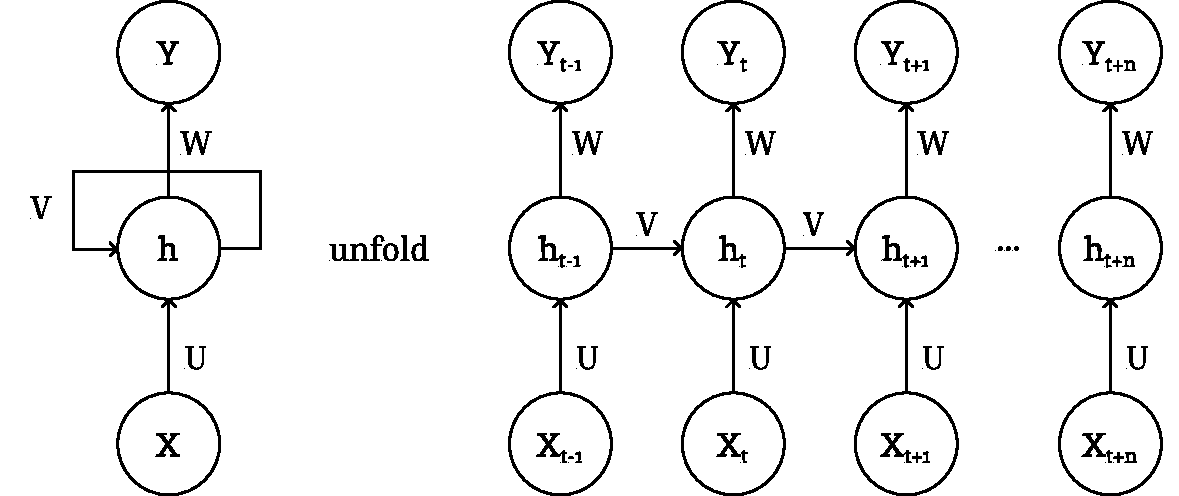
\includegraphics[width=0.8\linewidth]{img/rnn.pdf}
	\caption{Recurrent Neural Network}
	\label{fig:rnn}
\end{figure}

\noindent \newline
Eine wichtige Erweiterung der RNNs sind Long Short-Term Memory Networks (LSTMs). LSTMs wurden 
entwickelt, um die Herausforderungen von RNNs, insbesondere das Problem des verschwindenden 
Gradienten bei langen Sequenzen, zu überwinden. LSTMs behalten die grundlegenden Eigenschaften von 
RNNs bei, führen jedoch eine zusätzliche Struktur ein: den Zellzustand. Neben dem versteckten 
Zustand (hidden state), der bei traditionellen RNNs verwendet wird, haben LSTMs einen Zellzustand 
(cell state), der es ihnen ermöglicht, Informationen über längere Zeiträume hinweg zu bewahren und 
zu verarbeiten.

\noindent \newline
Dieser Zellzustand arbeitet als eine Art "Gedächtnis" der LSTM, das es ihm ermöglicht, sowohl 
kurzfristige als auch langfristige Abhängigkeiten in Daten zu erkennen und zu lernen. Dies ist 
besonders nützlich in Anwendungen wie der Spracherkennung oder der Vorhersage von Zeitreihen, wo 
die Beziehung von Datenpunkten über längere Zeiträume hinweg entscheidend ist. 
(\cite{weidman2019deep} Chapter 6).

\subsubsection{Metriken}
Neuronale Netze werden trainiert, um spezifische Ausgaben zu generieren. Zur Bewertung ihrer 
Performance dienen verschiedene Metriken, die in diesem Kapitel vorgestellt werden. Neben der bereits 
besprochenen Loss Function, die den Unterschied zwischen der tatsächlichen und der gewünschten 
Ausgabe quantifiziert, nutzen wir weitere Metriken. Die nachstehende Formel illustriert den 
\textit{Mean Squared Error} (MSE), eine gängige Methode, um den Loss zu berechnen:

\begin{equation*}
    \text{MSE} = \frac{1}{n} \sum_{i=1}^{n} (y_{i} - \hat{y}_{i})^{2}
\end{equation*}

\noindent
Vor der Betrachtung weiterer Metriken ist das Verständnis der \textit{Confusion Matrix} wesentlich. 
Sie veranschaulicht die Anzahl korrekter und inkorrekter Vorhersagen des Modells. In dieser Arbeit 
konzentrieren wir uns auf die Klassifizierung eines Triggerworts, für welche die Confusion Matrix 
in Tabelle \ref{tab:confusion_matrix} abgebildet ist.

\begin{table}[H]
	\centering
	\begin{tabular}{|c|c|c|}
		\cline{2-3}
		\multicolumn{1}{c|}{} & \multicolumn{2}{c|}{\textbf{Predicted}} \\ \hline
		\textbf{Actual}     & \textbf{Triggerwort} & \textbf{Kein Triggerwort} \\ \hline
		\textbf{Triggerwort} & True Positive (TP)   & False Negative (FN)       \\ \hline
		\textbf{Kein Triggerwort} & False Positive (FP)  & True Negative (TN)        \\ \hline
	\end{tabular}
	\caption{Confusion Matrix}
	\label{tab:confusion_matrix}	
\end{table}

\noindent \newline
Mit der Confusion Matrix können wir nun die anderen Metriken betrachten. Die \textit{Accuracy} 
zeigt den Anteil der korrekten Vorhersagen. Die Accuracy wird wie folgt berechnet:

\begin{equation*}
	\text{Accuracy} = \frac{TP + TN}{TP + TN + FP + FN}
\end{equation*}

\noindent \newline
Die \textit{Precision} zeigt den Anteil der korrekten positiven Vorhersagen. Die Precision wird wie 
folgt berechnet:

\begin{equation*}
	\text{Precision} = \frac{TP}{TP + FP}
\end{equation*}

\noindent \newline
Die \textit{Recall} zeigt den Anteil der korrekten positiven Vorhersagen. Die Recall wird wie 
folgt berechnet:

\begin{equation*}
	\text{Recall} = \frac{TP}{TP + FN}
\end{equation*}

\noindent  \newline
Die \textit{F1-Score} ist das harmonische Mittel zwischen Precision und Recall. Die F1-Score wird 
wie folgt berechnet:

\begin{equation*}
	\text{F1-Score} = 2 \cdot \frac{\text{Precision} \cdot \text{Recall}}{\text{Precision} + 
	\text{Recall}}
\end{equation*}

\newpage \section{Stand der Forschung}
Der Stand der Forschung ist ein wichtiger Teil dieser Arbeit. Darin werden die wichtigsten
zeitlichen Entwicklungen im Bereich der Spracherkennung dargestellt. Die Forschung im Bereich 
der Spracherkennung ist ein aktives Forschungsgebiet. Die Jahre 2010 bis 2020 haben laut 
(\cite{hannun2021history}) einen grossen Fortschritt in der Spracherkennung erlebt. Dieser 
Fortschritt ist vor allem auf die Verwendung von Deep Learning zurückzuführen.Weiter wird der 
Aufbau von Sprachassistenten untersucht und verglichen. Ein wichtiger Teil ist die Funktionsweise 
vom Sprachassistent Siri. Apple veröffentlichte seinen Sprachassistenten im Jahr 2011 mit dem 
Release von iOS 5. Weiter betrachten wir eine kommerzielle Lösung von Picovoice, welche aufzeigen 
soll, dass es einen Bedarf für eine integrierte Spracherkennungslösung gibt.

\subsection{Zeitliche Entwicklung der Spracherkennung}
Die Spracherkennung entwickelte sich von 2010 bis 2020 mit enormen Fortschritten. In der heutigen
Zeit wird die Spracherkennung in Form von Sprachassistenten wie Siri, Alexa und Google Assistant von
vielen Menschen genutzt. Die Nutzung der Sprachassistenten wird vor allem für Suchanfragen
verwendet. Angesichts des Fortschritts der letzten Jahre stellt sich die Frage, was die Zukunft
bringen wird (\cite{hannun2021history}).

\noindent \newline
Die Abbildung \ref{fig:updated_timeline} zeigt eine Timeline der wichtigsten Entwicklungen im
Zeitraum von 2010 bis 2020. Die Timeline wurde basierend auf der Timeline von
(\cite{hannun2021history}) erstellt aber mit einem Zusatz für das Jahr 2020, welches die neuste
Entwicklung von Facebook AI's wav2vec2 aufzeigt (\cite{baevski2020wav2vec}).

\begin{figure}[htb]
	\centering
	\begin{tikzpicture}[scale=1.5, every node/.style={scale=0.8}]
		% Drawing the horizontal line
		\draw[->, thick] (0,0) -- (10,0);
		\foreach \x in {0,10} {
				\draw (\x,-0.1) -- (\x,0.1);
			}

		\foreach \x [count=\xi] in {2010,...,2020} {
				\draw (\xi-1,-0.1) -- (\xi-1,0.1); % draws the tick mark
				% \node[below] at (\xi-1,-0.2) {\x}; % labels the tick mark
			}

		% Labeling
		\node[align=center, below] at (0,-0.8) {2010};
		\node[align=center, below] at (10,-0.8) {2020};

		% Events
		\node[align=center, above] (kaldi) at (1.25,0.5) {Kaldi};
		\node[align=center, above] (hybrid) at (2.4,1) {Hybrid\\HMM/DNN};
		\node[align=center, above] (deepspeech) at (4.75,0.5) {Deep\\Speech};
		\node[align=center, above] (librispeech) at (5.5,1) {LibriSpeech};
		\node[align=center, above] (googlehome) at (6.7,1) {Google\\Home};
		\node[align=center, above] (humanlevel) at (7.75,0.75) {Human-level\\Switchboard};
		\node[align=center, above] (wav2vec2) at (10.0,0.75) {Facebook AI\\wav2vec2};
		\node[align=center, below] (applesiri) at (1.6,-0.8) {Apple Siri};
		\node[align=center, below] (amazonecho) at (4.55,-0.5) {Amazon Echo};
		\node[align=center, below] (encoder) at (5.8,-1.175) {Encoder-decoder\\models for ASR};
		\node[align=center, below] (deepspeech2) at (6.75,-0.5) {Deep Speech 2};
		\node[align=center, below] (googletransducer) at (9,-1) 
		{Google streaming\\on-device transducer};

		% Lines to the events
		\draw (kaldi) -- (1.25,0.1);
		\draw (hybrid) -- (2.4,0.1);
		\draw (deepspeech) -- (4.75,0.1);
		\draw (librispeech) -- (5.5,0.1);
		\draw (googlehome) -- (6.7,0.1);
		\draw (humanlevel) -- (7.75,0.1);
		\draw (wav2vec2) -- (10.0,0.1);
		\draw (applesiri) -- (1.6,-0.1);
		\draw (amazonecho) -- (4.55,-0.1);
		\draw (encoder) -- (5.8,-0.1);
		\draw (deepspeech2) -- (6.75,-0.1);
		\draw (googletransducer) -- (9,-0.1);
	\end{tikzpicture}
	\caption{Timeline of Speech Recognition Developments (2010-2020)}
	\label{fig:updated_timeline} % for later references
\end{figure}

\noindent \newline

\noindent \newline
Deep Learning hat zum grossen Teilen die Spracherkennung revolutioniert, insbesondere durch die
Sammlung grosser transkribierter Datensätze und Fortschritte in der Hardware. Spätestens seit
(\textit{Deep Speech}) sind Fähigkeiten der akustischen Sprachmodelle mit denen von Menschen
vergleichbar (\cite{hannun2021history}).

\noindent \newline
Als offene Vorhersage für die Zukunft der Spracherkennung bezieht sich (\cite{hannun2021history})
auf die Entwicklung bis 2030. Bis 2030 wird die Spracherkennungs-Forschung eine Verlagerung zu
self-supervised Modellen und On-Device-Training erleben, wobei der Fokus auf kleine sparsame Modelle
und personalisierten Modellen liegt. Die Wortfehlerrate wird weiter sinken, während die
Sprachqualität steigt (\cite{hannun2021history}).

\subsection{Aufbau von Sprachassistenten}
Sprachassistenten können laut (\cite{matarneh2017speechrecognition}) in folgende Komponenten
unterteilt werden: Sprache, Erkennung, Übersetzung und Ausführung von Befehlen. Die nachfolgende
Abbildung \ref{fig:voice_control} zeigt die Komponenten eines Sprachassistenten. Abbildung basiert
auf (\cite{matarneh2017speechrecognition}). Zudem wurde aber die Komponente des \gls{twd} 
hinzugefügt.

\vspace{1em}
\begin{figure}[h!]
	\centering
	\begin{tikzpicture}[node distance=3.75cm, auto, thick, >=Latex]
		% Defining style for the blocks
		\tikzset{block/.style= {draw, rectangle, align=center, minimum width=2.5cm, 
		minimum height=1.25cm, font=\scriptsize}}
		% Nodes
		\node[block] (detector) {Trigger Word\\Detector};
		\node[block, right of=detector] (recognition) {Recognition of\\the speech};
		\node[block, right of=recognition] (translation) {Translation of speech\\into commands};
		\node[block, right of=translation] (execution) {Execution of\\commands};
		\node[block, left of=detector] (speech) {Speech};
		% Arrows
		\draw[->] (speech) -- (detector);
		\draw[->] (detector) -- (recognition);
		\draw[->] (recognition) -- (translation);
		\draw[->] (translation) -- (execution);
	\end{tikzpicture}	
	\caption{Voice control implementation.}
	\label{fig:voice_control}
\end{figure}

\noindent \newline
Sprachassistenten funktionieren mehrheitlich nach dem gleichen Prinzip. Die Sprache wird
durch ein Mikrofon aufgenommen und in ein digitales Signal umgewandelt. Das digitale Signal wird
durch einen Trigger Word Detector (TWD) analysiert. Der TWD erkennt, ob das gesprochene Wort die 
Erkennung aktivieren soll. Für die effektive \gls{asr} können verschiedene Ansätze verwendet
werden. Eine Möglichkeit ist einen Cloud-basierten Ansatz zu verwenden. Anbieter wie Google,
Amazon und Apple verwenden für ihre Sprachassistenten Cloud-basierte Ansätze 
(\cite{matarneh2017speechrecognition}). 

\subsection{Vergleich von Sprachassistenten}\label{sec:vergleich_sprachassistenten}

In der Arbeit von (\cite{matarneh2017speechrecognition}) werden verschiedene Spracherkennungssysteme 
anhand von Kriterien wie Genauigkeit, API-Qualität, Leistung, Echtzeitgeschwindigkeit, 
Antwortzeit und Kompatibilität verglichen. Die Beurteilung umfasst sowohl Systeme mit offenem 
(\textit{Open-Source}) als auch geschlossenem Sourcecode (\textit{Closed-Source}), mit einer 
detaillierten Untersuchung von deren Fähigkeiten und Einschränkungen.

\raggedcolumns
\begin{multicols}{2}
	\small 
	\setlength\itemsep{0em} 
	
	\noindent Closed-Source:
	\begin{itemize}[itemsep=0px, parsep=0px]
	\item Dragon Mobile SDK
	\item Google Speech Recognition
	\item SIRI
	\item Yandex SpeechKit
	\item Microsoft Speech API
	\end{itemize}
	
	\columnbreak
	
	\noindent Open-Source:
	\begin{itemize}[itemsep=0px, parsep=0px]
	\item CMU Sphinx
	\item Kaldi
	\item Julius
	\item HTK
	\item iAtros
	\item RWTH ASR
	\item Simon
	\end{itemize}
\end{multicols}
	
\noindent \newline
Zusammenfassend kann festgestellt werden, dass das Dragon Mobile SDK bei den Closed-Source-Systemen 
in Bezug auf Genauigkeit und Benutzerfreundlichkeit führend ist. Bei den Open-Source-Systemen 
sticht CMU Sphinx besonders hervor. Dennoch hat die Evaluation ergeben, dass aktuell keine der 
Systeme optimal und unkompliziert in mobile Apps integriert werden kann. Abgesehen von CMU Sphinx 
liegt der Schwerpunkt zudem nicht wirklich auf dem Trigger Word Spotting sondern auf der
Automatic Speech Recognition (ASR).

\subsection{Facebook AI wav2vec2}

Im Jahr 2020 präsentierte Facebook AI mit wav2vec2 ein innovatives Modell im Bereich der 
Spracherkennung. Dieses Modell stellt einen signifikanten Durchbruch in der Technologie dar und 
nutzt eine Methode, die als \textit{Self-Supervised Learning} bezeichnet wird. Durch diese Methode 
hat wav2vec2 das Potenzial, die Genauigkeit und Effizienz der Spracherkennung erheblich zu steigern 
(\cite{baevski2020wav2vec}).

\noindent \newline
Für die Zielsetzung dieser Arbeit bietet wav2vec2 eine vielversprechende Perspektive. Obwohl es 
primär nicht für die Triggerwort-Erkennung entwickelt wurde, besteht die Möglichkeit, eines seiner 
Basis-Modelle entsprechend zu adaptieren. Durch gezielte Anpassungen könnte wav2vec2 so modifiziert 
werden, dass es effektiv für die Triggerwort-Erkennung eingesetzt werden kann. Dies würde nicht nur 
die Genauigkeit der Erkennung verbessern, sondern auch die Effizienz des gesamten Systems steigern. 
Es lohnt sich daher, die Potenziale und Anpassungsmöglichkeiten von wav2vec2 für diese spezifische 
Anwendung weiter zu untersuchen.

\noindent \newline
Darüber hinaus zeigt wav2vec2.0 das grosse Potenzial des Vortrainierens auf nicht beschrifteten 
Daten für die Sprachverarbeitung. Selbst mit nur 10 Minuten beschrifteter Trainingsdaten erreicht 
das Modell beeindruckende Ergebnisse auf dem Librispeech-Test (\cite{baevski2020wav2vec}). Es stellt 
auch einen neuen Standard in der Librispeech-Benchmark für verrauschte Sprache dar und übertrifft 
Modelle, die mit 100 Stunden Daten trainiert wurden, obwohl es 100-mal weniger beschriftete Daten 
verwendet.

\noindent \newline
Für das Vorhaben dieser Arbeit könnte wav2vec2 von grossem Nutzen sein. Da es einen signifikanten
Durchbruch in der Technologie darstellt, könnte es die Genauigkeit und Effizienz der Spracherkennung
erheblich steigern. Es ist zwar im Bezug auf die Trigger Word Erkennung nicht direkt anwendbar, 
aber durch adaptieren eines der Basis Modelle könnte es umfunktioniert werden.


\newpage
\subsection{Funktionsweise von Siri}
Die Implementation von Siri ist nicht öffentlich zugänglich, aber Apple selbst dokumentiert
das Grundlegende Konzept von Siri sehr detailliert. Der Beitrag ``Hey Siri: An On-device DNN-powered
Voice Trigger for Apple’s Personal Assistant'' (\cite{siri2017hey}) von der ML Research Group von
Apple gibt einen sehr detaillierten Einblick in die Funktionsweise von Siri. Siri besteht aus
diversen Komponenten, welche mehrheitlich in der Cloud laufen. ``Most of the implementation of Siri
is in the Cloud, including the main automatic speech recognition, the natural language
interpretation and the various information services.'' (\cite{siri2017hey}). Der Trigger von Siri
läuft jedoch auf dem Gerät selbst. Um diesen geht es im wesentlichen in diesem Kapitel.

\noindent \newline
Siri verwendet für den Voice Trigger ein Deep Neural Network (DNN) um das akustische Muster jedes
Frames in eine Verteilung von Wahrscheinlichkeiten für jeden Phonem zu übersetzen. Die Phoneme sind
die Bausteine der akustischen Sprache. Aus den Wahrscheinlichkeiten wird in einen zeitlichen
Integrationsprozess bestimmt, wie sicher es ist, dass das Gesagte 'Hey Siri' war.

\noindent \newline
Das Mikrofon des Geräts wandelt das Audiosignal in einen kontinuierlichen Stream von 16000 Samples
pro Sekunde um. Diese Samples werden anschliessend durch eine Spektralanalyse in eine Abfolge von
Frames transformiert, wobei jeder dieser Frames das Spektrum von ungefähr 0,01 Sekunden beschreibt.
Zwanzig Frames, die sich über 0,2 Sekunden erstrecken, werden dann als Eingabe für das DNN
verwendet.

\noindent \newline
Die Architektur der für Siri verwendeten DNNs bestehen typischerweise aus fünf Layers. In der
nachfolgenden Abbildung \ref{fig:siri_dnn} ist die Architektur des DNNs dargestellt. Die Quelle der
Abbildung ist der Beitrag ``Hey Siri: An On-device DNN-powered Voice Trigger for Apple’s Personal
Assistant'' (\cite{siri2017hey}).

\begin{figure}[h]
	\centering
	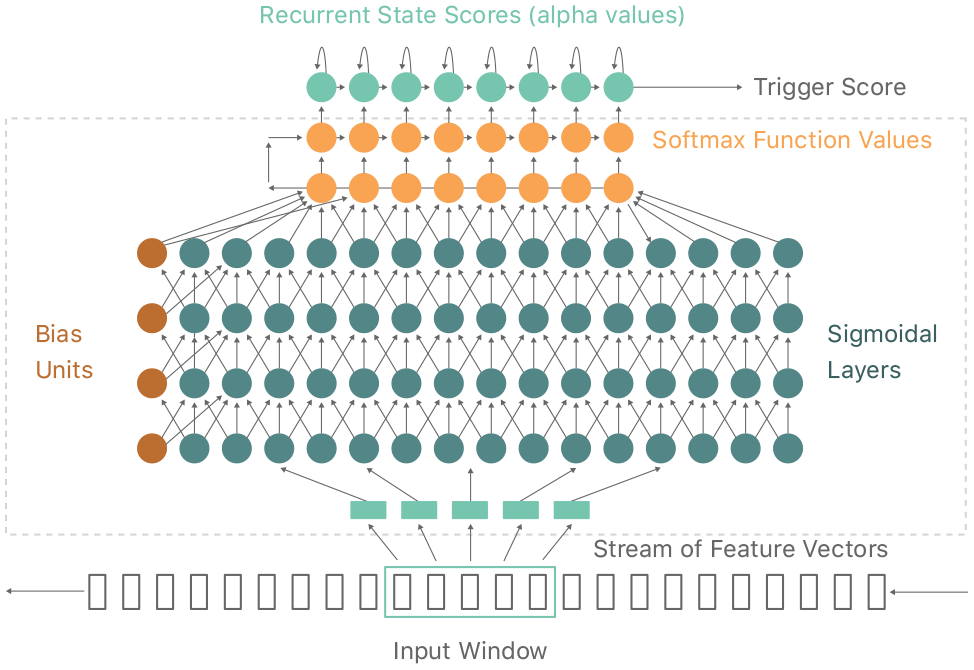
\includegraphics[width=0.75\linewidth]{img/siri_dnn.png}
	\caption{DNN Architektur von Siri}
	\label{fig:siri_dnn}
\end{figure}

\noindent
Die Siri DNNs werden je nach Gerätetyp und Leistung in verschiedenen Grössen implementiert.
Typische Hidden Layer Grössen sind 32, 128 oder 192. Bei Siri werden mehrheitlich fully-connected
Layers verwendet. Siri verwendet beim obersten Layer einen RNN Layer. Dies um die zeitliche
Abfolge der Frames zu berücksichtigen und basierend darauf einen Score zu berechnen. Siri verwendet
nicht nur ein Neuronales Netz, sondern gleich zwei. Das erste wird für die erste Erkennung von
'Hey Siri' verwendet. Das zweite dient als Bestätigung bzw. als zusätzlichen Checker.

\noindent \newline
Weiter wird im Beitrag ``Hey Siri: An On-device DNN-powered Voice Trigger for Apple’s Personal
Assistant'' (\cite{siri2017hey}) beschrieben, dass die Erkennung von 'Hey Siri' nicht nur schnell sein
muss, sondern auch sehr energieeffizient. Das folgende Zitat aus dem Beitrag beschreibt die
Anforderungen an die Erkennung von 'Hey Siri' sehr gut:

\begin{displayquote}
	``The Hey Siri detector not only has to be accurate, but it needs to be fast
	and not have a significant effect on battery life.''  (\cite{siri2017hey})
\end{displayquote}

\subsubsection{Takeaways}
Es ist sehr interessant zu sehen, wie der Trigger Mechanismus von Siri funktioniert. Der simple
Aufbau mit einem DNN, welches die Wahrscheinlichkeiten für jedes Phonem berechnet, ist sehr
interessant. Die Verwendung von zwei DNNs ist ebenfalls wertvoll und kann auch in dieser Arbeit
in Betracht gezogen werden. Ebenfalls wird die Notwendigkeit von einer schnellen und
energieeffizienten Erkennung von 'Hey Siri' deutlich. Dies ist auch für die Umsetzung dieser Arbeit
ein wichtiger Punkt. Die beiden Beiträge (\cite{siri2017hey}) und (\cite{apple2023voice}) geben
einen sehr guten Einblick in die Funktionsweise von Siri und sind essentiell für die Umsetzung
dieser Arbeit.


\subsection{Marktanalyse - Trigger Wort Erkennung}
Während der Recherche für diese Arbeit wurden bestehende Lösungen auf dem Markt gesucht. Nebst den 
bereits erwähnten Lösungen im Unterkapitel \ref{sec:vergleich_sprachassistenten} wurde eine Lösung 
gefunden. Es wurde ein Anbieter gefunden, welcher exakt eine Lösung für die Trigger Wort Erkennung 
anbietet. Der Anbieter heisst Picovoice und bietet eine Lösung mit dem Namen Porcupine an. Sie 
beschreiben ihre Lösung wie folgt:

\begin{displayquote}
	``Porcupine Wake Word is a wake word detection engine that recognizes unique signals to
	transition software from passive to active listening. Porcupine Wake Word enables enterprises
	to offer hands-free experiences by training and deploying custom wake words like Big Tech -
	but with superior technology.'' (\cite{picovoice2023porcupine})
\end{displayquote}

\noindent \newline
Porcupine verspricht eine sehr hohe Genauigkeit und eine sehr schnelle Erkennung. Ebenfalls bieten
sie eine grosse Auswahl an Integrationen für verschidenste Programmiersprachen bzw. Plattformen an.
Um nur einige zu nennen: Python, C, Flutter, Java, JavaScript, Android, iOS, NodeJS, Unity, React
und viele mehr. Die Integrationen sehen sehr vielversprechend aus und sind sehr einfach zu
implementieren. Bei den Preisen bietet Picovoice drei verschiedene Modelle an. Individuell,
Developer und Enterprise. Für ein grösseres Projekt mit dem Bedarf nach einer individuellen
Triggerwort Erkennung könnte es genau die richtige Lösung sein. Dennoch ist gilt es zu erwähnen,
dass die Lösung von Picovoice nicht Open Source ist. Die Preise sind ebenfalls nicht ganz ohne.
Die Enterprise Lösung startet bei 2'500 USD pro Monat und ist somit für viele Projekte nicht
finanzierbar. Die Preise sind auf der Webseite von Picovoice einsehbar
(\cite{picovoice2023porcupine}).



\subsection{Diskussion}
Die Trigger Wort Erkennung ist ein aktives Forschungsgebiet. Es gibt viele verschiedene Ansätze und
Lösungen. Die in diesem Kapitel betrachteten Lösungen und Ansätze haben einen guten Einblick in die
Funktionsweise von Trigger Wort Erkennung gegeben. Die Funktionsweise von Siri hat hierbei einen
besonderen Einblick gegeben.

\newpage \section{Ideen und Konzepte}
Dieses Kapitel beschreibt die Ideen und Konzepte, die für die Umsetzung der Arbeit verwendet
werden. Es wird auch auf die verwendeten Technologien eingegangen. Die Grob Idee ist es im 
wesentlichen, ein eigenes Modell zu trainieren, ganz nach dem Vorbild von (\cite{siri2017hey}), 
welches Triggerwörter erkennt. Dazu wird ein Datensatz erstellt, welcher die Triggerwörter, 
sowie andere Wörter enthält. Weiter sollen weitere Datensätze untersucht werden, um die 
Genauigkeit des Modells zu verbessern. Eines der gefundenen Datensätze ist der 
\textit{Mozilla Common Voice} Datensatz (\cite{ardila2020common}). Dieser Datensatz enthält 
unzählige Sprachaufnahmen von Menschen, welche freiwillig ihre Stimme aufgenommen haben. 

\subsection{Grundlegende Idee}
Um die Grundlegende Idee zu beschreiben wird die Abbildung \ref{fig:basic_idea} verwendet. Darin 
wird illustrativ dargestellt, wie die Grundlegende Idee umgesetzt werden soll. Es startet mit der
Erarbeitung der Grundlagen in Bezug auf Audio und Machine Learning. Danach wird eine Möglichkeit
erarbeitet, um Sprachaufnahmen zu machen. Ein Schritt weiter ist es, die Sprachaufnahmen
aufzubereiten und in ein Format zu bringen, welches für das Training eines Modells verwendet werden
kann. Ebenfalls soll eine Modelarchitektur erarbeitet werden, welche für die Triggerwort Erkennung
verwendet werden kann. Nachdem das Modell trainiert wurde, soll es in eine App integriert werden.

\begin{figure}[h]
	\centering
	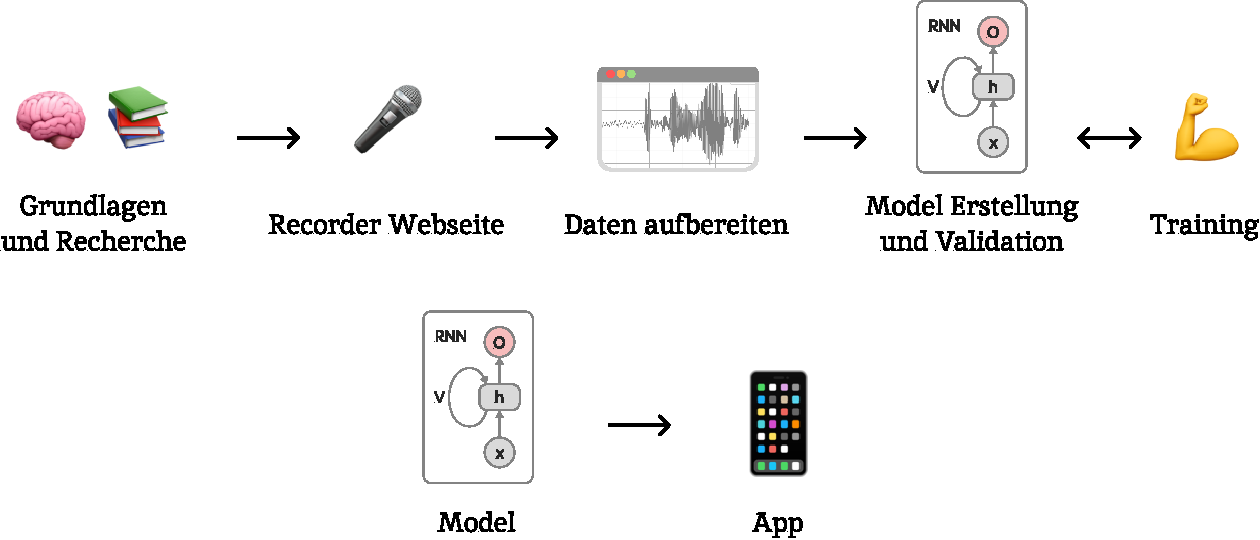
\includegraphics[width=0.85\linewidth]{img/basic_idea.pdf}
	\caption{Grundlegende Idee}
	\label{fig:basic_idea}
\end{figure}

\noindent \newline
Das Ergebnis soll eine App sein, welche ein Triggerwort erkennt. Das Resultat dieser Bachelorarbeit
ist sozusagen eine Teilkomponente einer Sprachsteuerung. Denn wie wir im Kapitel Stand der Forschung
gesehen haben, besteht eine Sprachsteuerung aus mehreren Komponenten. Um einen möglichen Use Case
zu nennen, könnte die App als Triggerwort Erkennung für eine Sprachsteuerung in einer Koch App
verwendet werden. Die App könnte dann beispielsweise folgende Befehle verstehen: ``Hey FOOBY, 
nächster Kochschritt'' oder ``Hey FOOBY, vorheriger Kochschritt''. Eine Sprachsteuerung für eine Koch App
würde somit den Anwendern ermöglichen, die Hände frei zu haben und sich voll und ganz auf das
Kochen zu konzentrieren. Die Nutzererfahrung könnte mit einem solchen Feature massiv verbessert
werden.

\subsection{Erstellung eines Datensatzes}
Die Erstellung eines Datensatzes ist ein wichtiger Bestandteil dieser Arbeit. Daher soll eine 
Möglichkeit erarbeitet werden, um Sprachaufnahmen zu machen. Der Datensatz soll aus Sprachaufnahmen
bestehen, welche Triggerwörter enthalten. Ebenfalls sollen die Sprachaufnahmen auch andere Wörter
enthalten. Neben den eigenen Sprachaufnahmen sollen auch bestehende Datensätze untersucht werden.

\noindent \newline
Ein sehr verbreiteter Datensatz ist der \textit{Mozilla Common Voice} Datensatz
(\cite{ardila2020common}). Dieser Datensatz enthält unzählige Sprachaufnahmen von Menschen, welche
freiwillig ihre Stimme aufgenommen haben. 

\subsection{Ethische Überlegungen}
Das Erstellen eines Datensatzes hat eine gewisse Verantwortung. Es geht dabei nicht nur um die 
Einhaltung des Datenschutzgesetzes, sondern auch um ethische Aspekte. Ein Datensatz sollte 
vielfältige Sprachaufnahmen beinhalten und nicht nur Aufnahmen bestimmter Personengruppen. Das 
Paper von Papakyriakopoulos et al. (\cite{papakyriakopoulos2023augmented}) betont die 
Notwendigkeit der Diversität in Sprachdaten und die Auswirkungen auf Fairness und Robustheit von 
Sprachtechnologien. Sie empfehlen, mehr Transparenz bei der Datensammlung zu schaffen, um ethische 
Aspekte zu dokumentieren und die Überlegungen zum sozialen Kontext der Datennutzung zu vertiefen.

\noindent \newline
In Bezug auf die Erstellung eines Datensatzes für diese Arbeit ist es beispielsweise wichtig, dass 
die Sprachaufnahmen aus diversen Sprachregionen stammen. In der Schweiz gibt es vier offizielle 
Sprachen und unzählige Dialekte. St. Galler Dialekt hat einen anderen Klang als der Zürcher Dialekt.
Ebenfalls gibt es Personen mit Sprachfehlern oder Personen, welche eine andere Sprache als 
Muttersprache haben. All diese Aspekte sollten bei der Erstellung eines Datensatzes berücksichtigt 
werden.

\subsection{Datenschutz und Privatsphäre}
Die Erestellung des Datensatzes und die Verwendung von Sprachaufnahmen soll unter Einhaltung des 
Datenschutzgesetzes erfolgen. Die Sprachaufnahmen sollen nicht an Dritte weitergegeben werden. Die 
Teilnehmer sollen über die Verwendung der Sprachaufnahmen informiert werden. Ebenfalls sollen die 
Sprachaufnahmen nach der Verwendung gelöscht werden. 

\subsection{Erste Überlegungen zu Tools und Technologien}
Für die Entwicklung von Machine-Learning-Modellen stehen mehrere Frameworks zur Verfügung. Eine 
Schlüsselüberlegung für dieses Projekt war die Fähigkeit zur Integration in eine mobile App.
Es gibt einge Frameworks, welche das ermöglichen. Um nur einige zu nennen: PyTorch, TensorFlow, 
CoreML. Wobei CoreML nur für Apple Ekosysteme verwendet werden kann. Da nicht nur die Integration
in eine mobile App wichtig ist, sondern auch die Entwicklung von Prototypen, wurde PyTorch gewählt.
TensorFlow wäre ebenfalls eine gute Wahl gewesen, aber laut (\cite{valantis2023battle}) hat PyTorch 
in den letzten Jahren an Popularität gewonnen. Ebenfalls ist PyTorch sehr beliebt für die 
Forschung und bietet eine Integration in mobile Apps. Daher wurde PyTorch als Framework für die 
Entwicklung der hier beschriebenen Arbeit gewählt.

\subsection{Erste Überlegungen zur Modelarchitektur}
Mit der Wahl von PyTorch als Framework wurde zwar eine wichtige Entscheidung getroffen, aber die 
Modelarchitektur ist noch nicht definiert. Die Inspiration für die Modelarchitektur kommt von 
(\cite{siri2017hey}). Die Modelarchitektur von Siri ist sehr einfach und besteht aus einem DNN. 
Daher war ein erster Gedanke, eine ähnliche Architektur zu verwenden. Im folgenden werden die 
unterschiedlichen Versuche die im Rahmen dieser Arbeit gemacht wurden, beschrieben. Als Experiment 
stand immer die Erkennung von 'Hey FOOBY' im Vordergrund.

\subsection{Versuche}
Als Teil der Ideen und Konzepte wurden verschiedene Versuche beziehungsweise Experimente gestartet. 
Diese Versuche sind wichtig, um die Machbarkeit der Triggerwort Erkennung zu überprüfen. Da aus dem 
Kapitel Stand der Forschung hervorgeht, dass das Model wav2vec2 von Facebook AI einen grossen 
Fortschritt in der Spracherkennung darstellt, basieren die ersten drei Versuche auf der Verwendung 
von wav2vec2.


\subsubsection{Versuch 1: Facebook AI wav2vec2}
Die ersten Versuche befassten sich mit der Verwendung von Facebook AI's wav2vec2. Dieses Modell 
ist zwar nicht für die Triggerwort Erkennung entwickelt worden, aber es hat das Potenzial diese 
Aufgabe zu erfüllen. Daher wurde ein Versuch gestartet, um zu sehen, ob es möglich ist mit wav2vec2 
Triggerwörter zu erkennen. Die folgende Abbildung \ref{fig:wav2vec2_code} zeigt den Code 
für die Verwendung von wav2vec2. 

\begin{figure}[h]
	\centering
	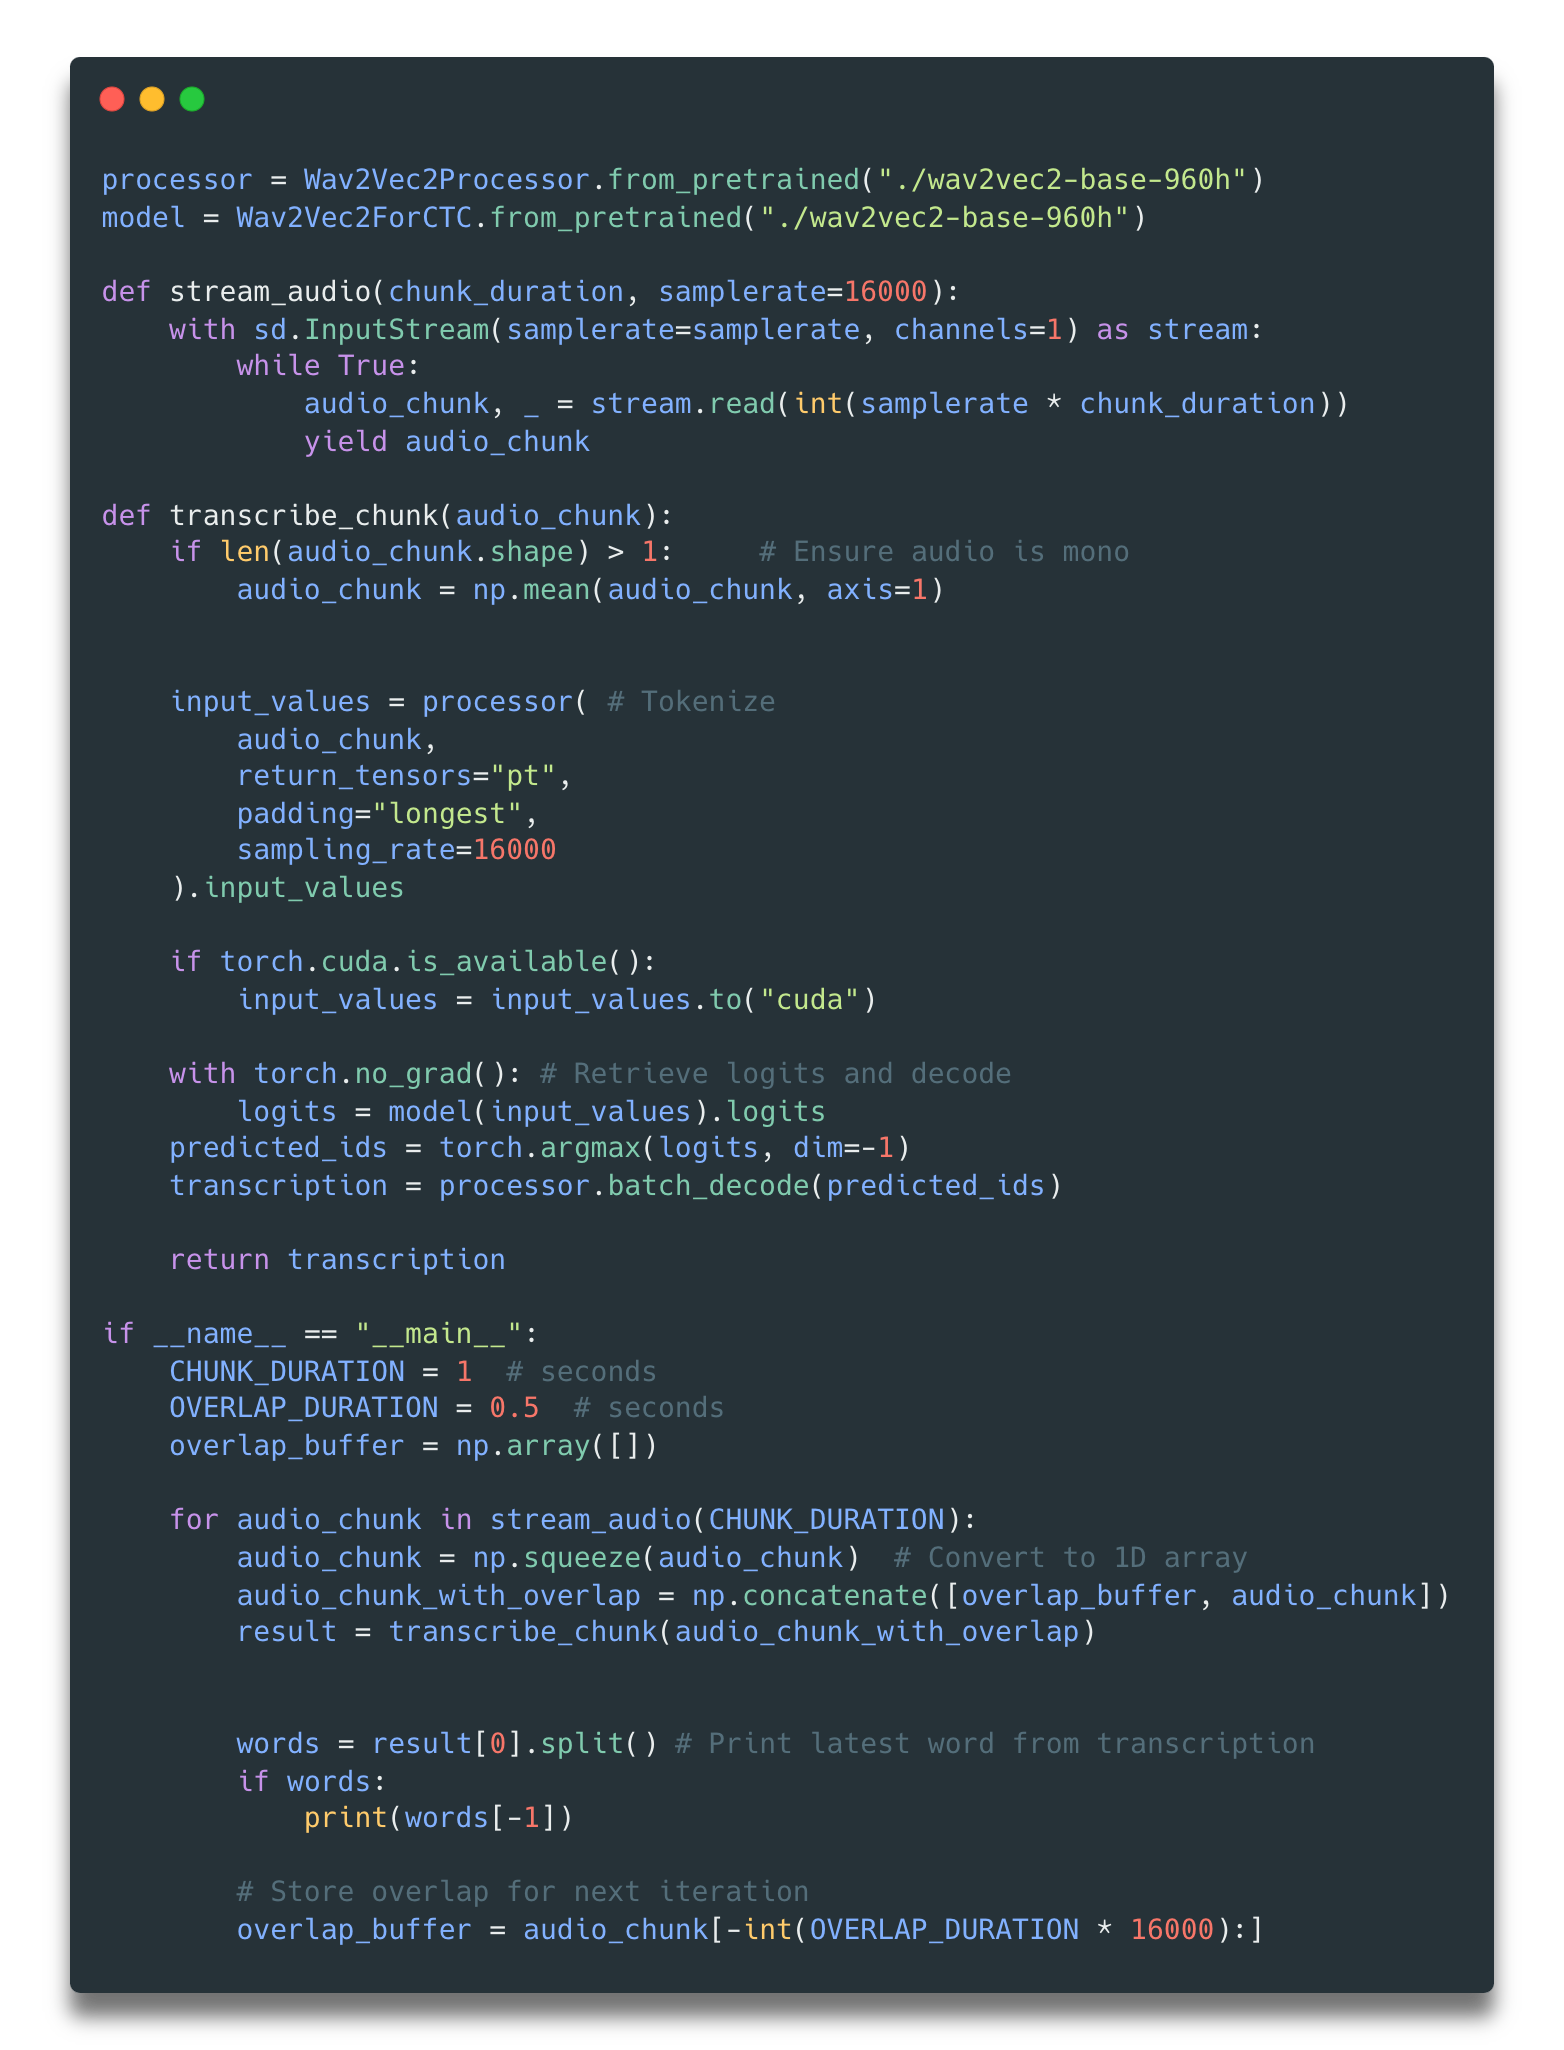
\includegraphics[width=0.75\linewidth]{img/wav2vec2_code.png}
	\caption{Verwendung von wav2vec2}
	\label{fig:wav2vec2_code}
\end{figure}

\noindent \newline
Die ersten Versuche mit wav2vec2 zeigten, dass es möglich ist, Triggerwörter zu erkennen, auch 
wenn es sich um ein Basismodell handelt, das noch nicht auf eine spezifische Aufgabe zugeschnitten 
wurde. In einer Testreihe mit drei 10-sekündigen Tests, in dem die Wörter "Hey FOOBY" mehrmals 
gesagt wurden, erkannte das Modell verschiedene Triggerwörter. Die zeitliche Abfolge dieser 
Erkennungen ist in Tabelle \ref{tab:wav2vec2_results} dargestellt.

\begin{table}[H]
	\centering
	\begin{tabular}{|c|c|c|c|}
		\hline
		\textbf{Zeitabschnitt} & \textbf{Test 1} & \textbf{Test 2} & \textbf{Test 3} \\
		\hline
		0-2s & FOOBY & HEY FOOBE & E FOOBE \\
		2-4s & F & B FOBE & E HA \\
		4-6s & FHOBI & HEY & FUBI \\
		6-8s & BE & FOOBE & HAL FUBI\\
		\hline
	\end{tabular}
	\caption{Resultate der ersten Versuche mit wav2vec2}
	\label{tab:wav2vec2_results}
\end{table}

\noindent \newline
Diese Versuche haben gezeigt, dass es möglich ist ähnliche Wörter zu erkennen. Auch wenn die 
Resultate in erster Linie nicht sehr gut erscheinen, sind sie dennoch vielversprechend. Als 
Beispiel könnten die Wörter 'Hey FOOBY' und 'Hey FOOBE' als ähnliche Wörter betrachten werden. 
Durch die Berechnung der Levenshtein-Distanz könnte die Ähnlichkeit dieser Wörter berechnet werden.
Die Levenshtein-Distanz ist eine Metrik zur Berechnung der Ähnlichkeit zweier Zeichenketten. Dieser 
Ansatz wurde jedoch nicht weiter verfolgt und stammt aus eigenen Überlegungen.

\subsubsection{Versuch 2: Fine-Tuning des Facebook AI wav2vec2-Modells}
Nach ersten Versuchen mit wav2vec2 wurde ein weiterer Ansatz verfolgt, der als Fine-Tuning bekannt 
ist. Hierbei wird ein bereits vortrainiertes Modell als Ausgangspunkt genutzt, welches dann für 
spezifische Aufgaben weiterentwickelt wird. Dies reduziert den ökologischen Fussabdruck durch 
geringeren Rechenaufwand (\cite{huggingface2023finetune}). Der Versuch umfasste die Anpassung des 
Basismodells durch Hinzufügen eines Layers, um das spezifische Triggerwort in Audio zu erkennen. 

\noindent \newline
Das `TriggerWordWav2Vec2Model` im Source Code \ref{fig:wav2vec2_finetune} erweitert das 
wav2vec2-Modell um ein Sequential Layer. Diese Komponente besteht aus einem Linear Layer, welcher 
den Output des wav2vec2-Modells verarbeitet, und einer Sigmoid Activation Function. Der Linear 
Layer verarbeitet die Average Pooling-Repräsentation der Hidden States des wav2vec2-Modells, um zu 
entscheiden, ob das Triggerwort in der Audioeingabe vorhanden ist oder nicht. So die Grundidee.

\begin{lstlisting}[caption={TriggerWordWav2Vec2Model}, label=fig:wav2vec2_finetune]

class TriggerWordWav2Vec2Model(nn.Module):
	def __init__(self, config):
		super(TriggerWordWav2Vec2Model, self).__init__()
		self.wav2vec2 = Wav2Vec2ForCTC(config).wav2vec2
		self.classifier = nn.Sequential(
			nn.Linear(config.hidden_size, 1),
			nn.Sigmoid()
		)

	def forward(self, input_values):
		transformer_outputs = self.wav2vec2(input_values).last_hidden_state
		avg_pool = transformer_outputs.mean(dim=1)
		return self.classifier(avg_pool)

\end{lstlisting}

\noindent \newline
Im Forward-Durchlauf des Modells werden die Audioeingaben durch das wav2vec2-Modell verarbeitet, 
das dabei relevante Merkmale aus den Audiodaten extrahiert. Vom Output des wav2vec2-Modells wird 
der Durchschnitt der Hidden States berechnet. Danch wird der Durchschnitt dem Linear Layer 
übergeben, welcher die Wahrscheinlichkeit berechnet, dass das Triggerwort in der Audioeingabe
vorhanden ist. Die Wahrscheinlichkeit wird durch die Sigmoid Activation Function berechnet. Der 
Prozess wird im Beitrag "Fine-tuning XLS-R for Multi-Lingual ASR with Transformers" von Patrick 
von Platen beschrieben:

\begin{displayquote}
	``For fine-tuning, a single linear layer is added on top of the pre-trained network to train 
	the model on labeled data of audio downstream tasks such as speech recognition, speech 
	translation and audio classification'' 
	(\cite{platen2021finetune})
\end{displayquote}

\noindent \newline
Dieser Ansatz ermöglicht eine effiziente und zielgerichtete Anwendung des vortrainierten 
wav2vec2-Modells für die spezifische Aufgabe der Triggerwort-Erkennung. Es nutzt die 
fortschrittlichen Fähigkeiten des wav2vec2-Modells zur Merkmalsextraktion und kombiniert 
diese mit einem massgeschneiderten Klassifikationsmechanismus, um hohe Genauigkeit bei der 
Erkennung von Triggerwörtern zu erreichen. Dennoch wurde dieser Ansatz nicht weiter verfolgt, da 
das resultierende Modell nicht den Anforderungen entsprechen in Bezug auf die Integration in eine 
mobile App. Es ist zum einen zu gross in Bezug auf der Grösse in Megabytes und zum anderen zu 
energieintensiv beziehungsweise zu rechenintensiv in der Inferenz. 



\subsubsection{Versuch 3: LiteFEW}
Nach den Misserfolgen mit wav2vec2 wurde ein weiterer vielversprechender Versuch gestartet. Dieser 
basiert auf dem Paper von lim et al. (\cite{lim2023lightweight}). Der Grundgedanke dieses Papers 
ist es, ein Modell auf Basis von wav2vec2 zu entwickeln, welches optimiert ist für die Triggerwort 
Erkennung auf mobilen Geräten. Das im Paper beschriebene Verfahren beinhaltet die Verwendung von 
wav2vec2 als Teacher-Model und ein kleineres Modell als Student-Model. Dieses Verfahren hätte 
den Vorteil die Problematik der im Versuch 2 beschriebenen Lösung zu umgehen. Doch an dieser Stelle 
wurde der Versuch abgebrochen, da die Implementation des Papers sehr komplex ist und kein Code 
veröffentlicht wurde.

\subsubsection{Versuch 4: ConvLSTM}
Nach den Misserfolgen mit wav2vec2 und LiteFEW war die Situation etwas frustrierend. Daher wurde 
ein weiterer Versuch gestartet, um ein eigenes Modell zu entwickeln. Dieser Versuch basiert auf 
dem Github Repository von Barazanji et al. (\cite{barazanji2023heyditto}). Das Github Repository 
enthält eine Definition für ein Modell, welches mit TensorFlow implementiert wurde. Das von 
Barazanji et al. (\cite{barazanji2023heyditto}) entwickelte Modell wurde für die Triggerwort 
Erkennung entwickelt und kann die Wörter 'Hey Ditto' erkennen. Ein Kritikpunkt an das Repository 
ist, dass es keine Dokumentation oder Quellenangaben enthält. Dennoch wurde das Modell als 
Grundlage für einen weiteren Versuch verwendet. Dazu wurde es in PyTorch übersetzt und 
entsprechend angepasst, sodass es auf den Anwendungsfall dieser Arbeit zugeschnitten ist. 
Das Verfahren selbst ist sehr interessant und basiert auf der Verwendung von Convolutional Layers 
in Kombination mit einem LSTM Layer. Hier konnte eine weitere Quelle gefunden werden, welche 
diese Art von Modelarchitektur verwendet. Das Paper von Khamees et al. 
(\cite{khamees2021classifying}) beschreibt das Klassifizieren von Musik Genres mit einer 
ähnlichen Modelarchitektur. Eine detailierte Beschreibung der Modelarchitektur ist im Kapitel der 
Realisierung zu finden.

\newpage \section{Methoden}
Das Vorgehen dieser Arbeit kann als eine klassische Projektvorgehen beschrieben werden. Aus der 
Aufgabenstellung ging schon hervor, dass ein eigenes Machine Learning Modell für die Triggerwort 
Erkennung erarbeitet werden soll. Zum andren soll das Modell in eine mobile App integriert werden.
Diese zwei Bereiche wurden Bereits bei der Planung der Arbeit definiert und haben daher die 
Planung der Arbeit stark beeinflusst.

\subsection{Projektphasen}
Im Projektmanagement wurden die Projektphasen definiert. Diese bestehen aus vier Phasen. Die erste
Phase widmet sich der \textit{Stand der Forschung}. Darin wurden aber bereits einige Punkte der 
Planung definiert sowie dem Setup der Entwicklungsumgebung. Der Bestandteil liegt aber in der 
Erarbeitung der Grundlagen sowie der Recherche von bestehenden Lösungen. Die zweite Phase ist die 
\textit{Erstellung des Modells}. In dieser Phase wird das Modell entwickelt, trainiert und 
evaluiert. Ebenfalls wird auch eine Möglichkeit erarbeitet um ein Datenstaz zu erstellen. In der 
dritten Phase namens \textit{Prototype} wird das Modell in eine mobile App integriert. 
Die letzte Phase ist das \textit{Refinement}. In dieser Phase wird die Arbeit sowie die
Dokumentation fertiggestellt. 

\subfile{projectmanagement.tex} % Projektmanagement separat

\newpage \section{Realisierung}
Die Realisierung dieser Arbeit besteht im wesentlichen aus drei Teilen. Welche die Ziele der Arbeit 
wiederspiegeln. Zum einen wurde ein Datensatz nach ethischen sowie rechtlichen Aspekten erstellt, 
welcher die Grundlage für die Experimente so wie das Training des Modells bildet. Weiter wurde ein 
Modell erarbeitet und anschliessend trainiert, welches Triggerwörter erkennt. Der letzte Teil der 
Realisierung ist die Integration dieses Modells in eine Sample App.

\subsection{Aufbau des Datensatzes}
Der Aufbau eines Datensatzes war zu Beginn der Arbeit geplant. Es war klar, dass ein Datensatz 
benötigt wird, um ein Modell zu trainieren. Der Datensatz wiederspiegelt die Grundlage des 
Problemfeldes. Es geht ja darum ein spezifisches Wort oder Wörter zu erkennen. Die nachfolgende 
Abbildung \ref{fig:dataset} zeigt die zwei Klassen des Datensatzes. Die Klasse 0 beinhaltet 
Sprachaufnahmen, welche das Triggerwort nicht enthalten. Die Klasse 1 beinhaltet Sprachaufnahmen, 
welche das Triggerwort enthalten.

\hspace*{-1.5cm}
\begin{figure}[h]
	\centering
	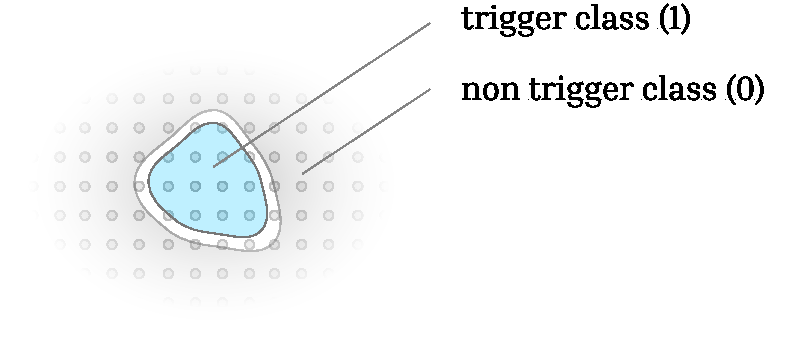
\includegraphics[width=0.75\linewidth]{img/dataset.pdf}
	\caption{Aufbau des Datensatzes}
	\label{fig:dataset} 
\end{figure}

\subsubsection{Recorder Webseite}
Um den Datensatz zu erstellen, wurde eine Webseite entwickelt, welche die Aufnahme von Sprachsamples 
ermöglicht. Die Webseite wurde auf Google Cloud Platform (GCP) gehostet, um eine zuverlässige und
skalierbare Lösung zu gewährleisten. Die Webseite wurde dockerisiert, was die Bereitstellung und 
Skalierung erleichtert. Zudem wurde sie auf den neuesten Stand gebracht, um sicherzustellen, dass 
sie mit aktuellen Technologien kompatibel ist. Bei der zugrunde liegenden Anwendung handelt es sich 
um eine Python Flask App, die für ihre Leichtigkeit und Flexibilität bekannt ist. Die Webseite 
stellt ein nützliches Tool dar, das die Aufnahme von Sprachsamples ermöglicht. Ursprünglich von 
Pete Warden entwickelt, bietet sie eine einfache und effiziente Möglichkeit, Sprachdaten zu sammeln 
(\cite{warden2018speech}).

\noindent \newline
Die Anpassungen der Webseite für diese Arbeit umfassten die folgenden Punkte:

\begin{itemize}
    \item \textbf{Hosting auf GCP}: Die Webseite wurde auf Google Cloud Platform (GCP) gehostet, um 
	eine zuverlässige und skalierbare Lösung zu gewährleisten.
    \item \textbf{Dockerisierung und Aktualisierung}: Die Anwendung wurde dockerisiert, was die 
	Bereitstellung und Skalierung erleichtert. Zudem wurde sie auf den neuesten Stand gebracht, um 
	sicherzustellen, dass sie mit aktuellen Technologien kompatibel ist.
    \item \textbf{Technische Details}: Bei der zugrunde liegenden Anwendung handelt es sich um eine 
	Python Flask App, die für ihre Leichtigkeit und Flexibilität bekannt ist.
    \item \textbf{Anpassungen für die Bachelorarbeit}: Die Zielwörter und die Länge der Aufnahmen 
	wurden modifiziert, um den spezifischen Anforderungen dieser Arbeit gerecht zu werden. Darüber 
	hinaus wurde die Webseite nahtlos in das Repository dieser Bachelorarbeit integriert.
\end{itemize}

\noindent \newline
Mit der überarbeiteten Recorder Webseite wurden Sprachaufnahmen von zwei Sekunden Länge und einer 
Sample Rate von 48kHz erstellt. Bei den freiwilligen Teilnehmern handelte es sich um Personen aus 
dem Bekanntenkreis des Autors. Um den Datenschutz zu gewährleisten, wurden die Teilnehmer über die 
Nutzung der Sprachaufnahmen informiert. Das Paper von Papakyriakopoulos et al. 
(\cite{papakyriakopoulos2023augmented}) betont die Notwendigkeit der Diversität in Sprachdaten. Die 
Aufnahmen beinhalten Aufnahmen von mindestens 10 verschiedenen Personen. Da die Variation der 
Sprachaufnahmen relativ gering war, wurden zusätzlich Augmentierungen der Sprachaufnahmen 
durchgeführt. Diese werden im Kapitel \ref{sec:augmentierung} beschrieben. Die nachstehende 
Abbildung gibt einen visuellen Überblick über das Erscheinungsbild und die Funktionalität der 
Webseite.

\begin{figure}[h]
    \centering
    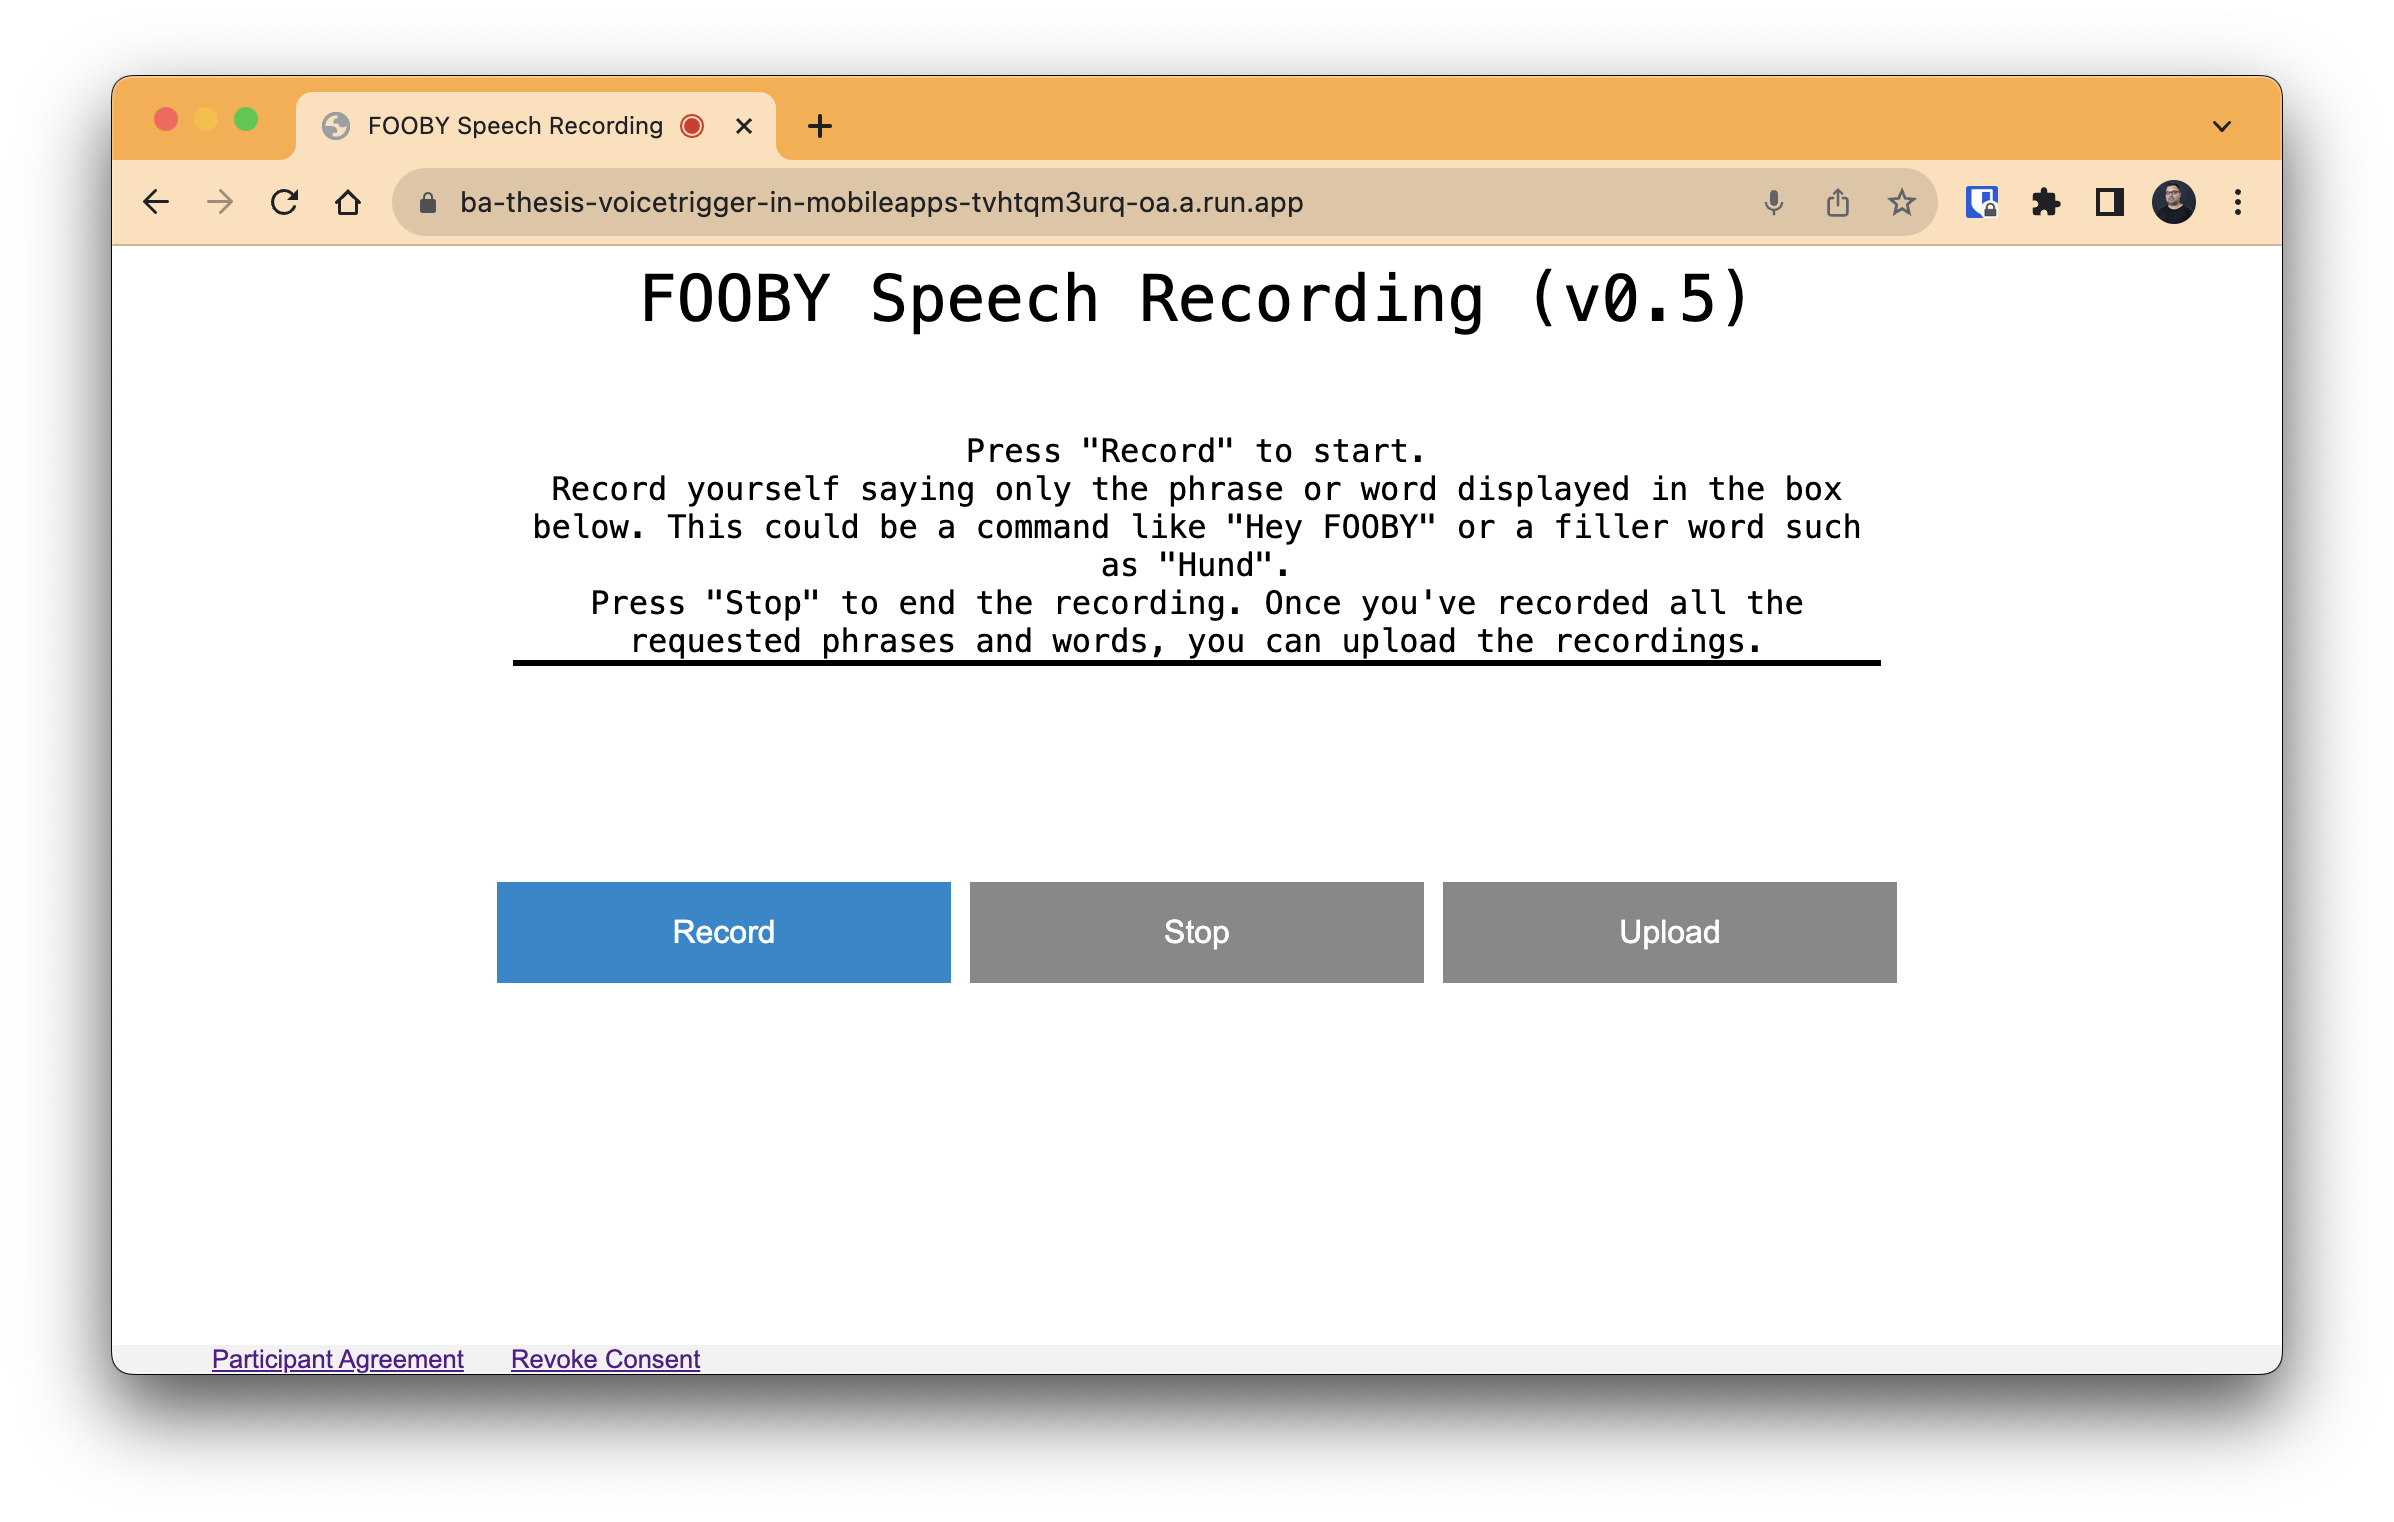
\includegraphics[width=0.8\textwidth]{img/ba-recorder-website.png} 
    \caption{Die überarbeitete Recorder Webseite}
    \label{fig:recorder_webseite}
\end{figure}

\subsubsection{Google Cloud Platform als Unterstützung}
Die Google Cloud Platform (GCP) ist eine Sammlung von Cloud Computing-Diensten. In dieser Arbeit
wurde die GCP verwendet, um die Recorder Webseite zu hosten. Ebenfalls wurde in betracht gezogen,
die Modelle auf der GCP zu trainieren. Die GCP bietet Services für Machine Learning an. Eines der
Services ist Vertex AI. Darin können beispielsweise Jupiter Notebooks verwendet werden, um Modelle
zu trainieren. Das Training kann beispielsweise auf CUDA-fähigen GPUs ausgeführt werden.

\noindent \newline
Die Sprachdaten wurden auf Google Cloud Storage (GCS) gespeichert. GCS ist ein Objektspeicher, der
für die Speicherung und Verteilung von grossen Datenmengen optimiert ist. Die Sprachdaten wurden
in einem Bucket gespeichert. Um mit der Datenschutzverordnung konform zu sein, wurde eine 
Löschrichtlinie für die Sprachdaten erstellt. Art. 17 Abs. 1 DSGVO besagt, dass Daten gelöscht 
werden müssen, wenn sie für den ursprünglichen Zweck nicht mehr erforderlich sind. Die
Löschrichtlinie wurde so konfiguriert, dass die Sprachdaten nach einem Jahr gelöscht werden.


\subsubsection{Augmentierung der Sprachdaten} \label{sec:augmentierung}
Um die Diversität und Robustheit der Sprachaufnahmen zu erhöhen und das Modell für die Erkennung 
von Triggerwörtern zu stärken, wurden gezielte Augmentierungstechniken eingesetzt. Dabei kamen 
Pitch Shifting zur Variation der Tonhöhe, Time Shifting zur Simulation zeitlicher Verschiebungen, 
Volume Control für Lautstärkeanpassungen und Noise Injection zur Ergänzung von 
Hintergrundgeräuschen zum Einsatz. Diese Massnahmen zielen darauf ab, die Generalisierungsfähigkeit 
des Modells zu verbessern und seine Leistung unter verschiedenen akustischen Bedingungen zu 
optimieren. Die Verwendung von Datenaugmentierung hat sich insbesondere bei einer begrenzten 
Anzahl von Samples als wirkungsvoll erwiesen und ist eine etablierte Methode in der Praxis. In 
Anlehnung an das Paper von Salamon et al. (\cite{salamon2017deep}), das den Einsatz verschiedener 
Augmentierungstechniken zur Verbesserung der Klassifikation von Umgebungsgeräuschen diskutiert, 
wurde das vorgeschlagene Verfahren angepasst, um die Herausforderungen bei der Erkennung von 
spezifischen akustischen Signalen, wie Triggerwörtern, zu meistern. Die effektive Kombination 
dieser Techniken im Trainingsprozess führte zu einem erweiterten und robusten Datensatz, der für 
die Entwicklung eines leistungsfähigen Erkennungssystems unerlässlich ist.


\subsubsection{Datensatz 'hey-fooby'}
Insgesamt wurden etwa 700 Sprachaufnahmen mit dem Recorder erstellt. 300 davon enthielten das 
Triggerwort 'Hey FOOBY', und 400 Aufnahmen bestanden aus anderen Wörtern. Durch 
Augmentierungstechniken wurde die Anzahl der Samples auf 10'000 erhöht, wobei ein Verhältnis von 
1 zu 2 im Vergleich zum 'other' Datensatz beibehalten wurde. Die daraus resultierende 
Imbalance wurde bei dem Training der finalen Modellarchitektur berücksichtigt.

\subsubsection{Datensatz 'other'}
Der 'other' Datensatz umfasst Sprachaufnahmen, die andere Wörter als das Triggerwort beinhalten. 
Von den ursprünglich 400 Aufnahmen wurde die Menge durch Augmentierung und die Integration 
weiterer Datensätze, darunter auch solche von Mozilla Common Voice (\cite{ardila2020common}), 
erhöht. Während des Trainings stellte sich heraus, dass das Modell auf Silence nicht adäquat 
reagierte, was die nachträgliche Hinzufügung von Silence Samples zum 'other' Datensatz motivierte. 
Gleiches galt für das Hinzufügen von Noise Samples, um die Reaktion auf Hintergrundgeräusche zu 
verbessern.


\newpage

\subsection{Erstellung des Modells}
Bei der Erstellung des Modells wurde die Architektur von Barazanji et al. 
(\cite{barazanji2023heyditto}) verwendet. Das Modell wurde in PyTorch implementiert als ein PyTorch 
Modul und anschliessend trainiert. Das Training wurde auf einem MacBook Pro mit einem M1 Pro Chip 
durchgeführt. Die Trainingszeit betrug für 120 Epochen etwa 8 Stunden. Neben der Architektur und 
dem Training des Modells wurde ebenfalls die Implementierung in einer Echtzeitanwendung konzipiert. 
Dabei war zu berücksichtigen, dass das Modell in eine mobile App integriert werden soll, weshalb 
besonderer Wert auf eine energieeffiziente Inferenz gelegt wurde. Die Echtzeitanwendung, entwickelt 
in Python, diente dazu, die Inferenzgeschwindigkeit des Modells zu testen, diese zu optimieren und 
entsprechende Leistungsmessungen durchzuführen.


\subsubsection{Verwendete Architektur des Modells}
Die Architektur besteht aus drei Convolutional Layers und einem Long-Short-Term-Memory 
(LSTM) Layer. Der Vorteil dieser Architektur ist, dass sie sehr energie effizient ist, wie auch sehr 
schnell in der Inferenz. Mehr dazu im Kapitel \ref{sec:evaluation}. Was besonders Markant ist, ist 
die Verwendung von Convolutional Layers in Kombination mit einem (LSTM) Layer, welcher die zeitliche 
Komponente der Sprache berücksichtigt. Die Idee der Kombination von Convolutional Layers und
(LSTM) Layers ist nicht neu. Es gibt diverse Paper, welche diesen Ansatz verwenden. Beispielsweise 
verwendet (\cite{khamees2021classifying}) diesen Ansatz für die Klassifizierung von Music Genres.
Die finale Architektur des Models ist in der Abbildung \ref{fig:model_architecture} dargestellt.
Für den Namen des Models wurde der Name \textit{WakeupTriggerConvLSTM2s} gewählt. Der Name 
beinhaltet information darüber, welche Architektur verwendet wurde. Die Zahl 2s steht für die 
Anzahl Sekunden, welche das Model analysiert. Die Abbildung wurde mit Figma und Blender erstellt.

\begin{figure}[h]
	\centering
	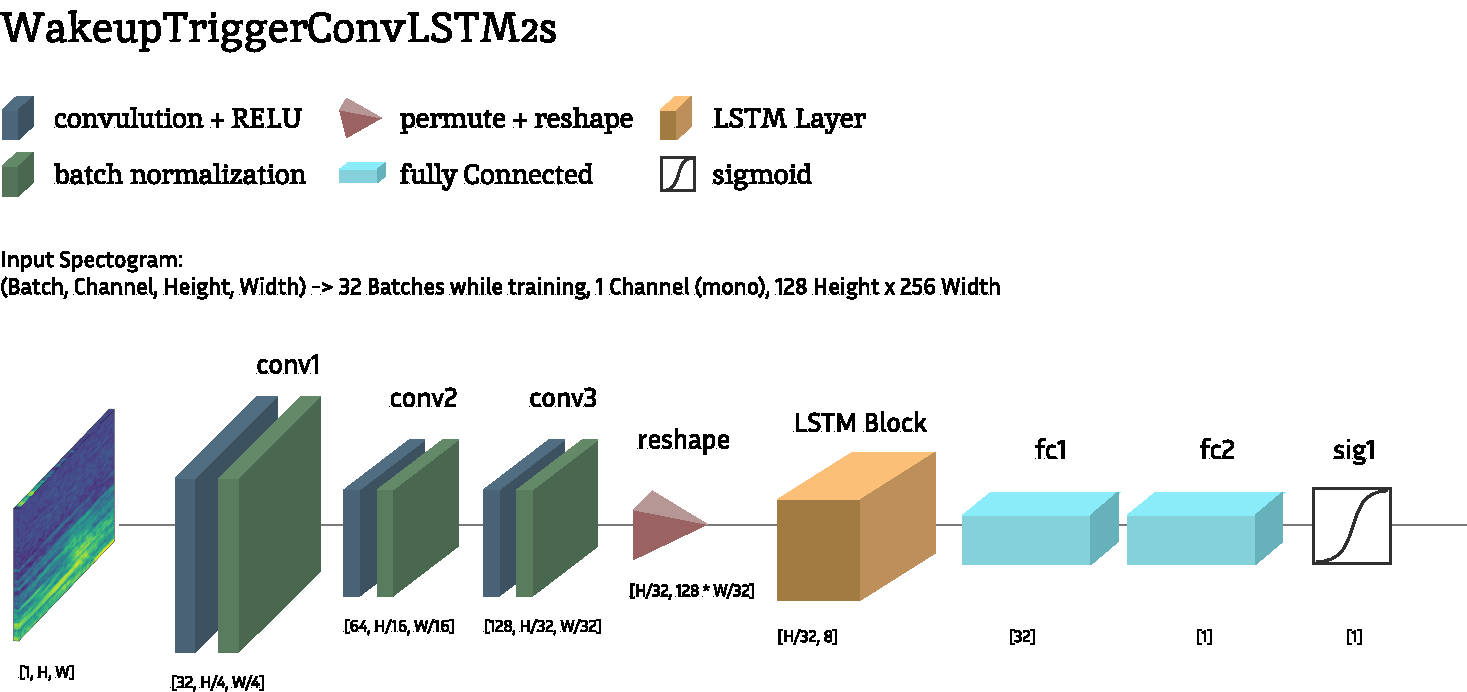
\includegraphics[width=1.0\linewidth]{img/model_architecture.pdf}
	\caption{Architektur des Modells}
	\label{fig:model_architecture}
\end{figure}

\noindent \newline
Diese Art von Modelarchitektur setzt eine Transformation der Sprachdaten in ein Spektrogramm voraus.
Die Transformation der Sprachdaten wurde im Kapiel \ref{sec:grundlagen} der Grundlagen bereits
beschrieben und wird im anschliessenden Kapitel nochmals genauer beschrieben.


\subsubsection{Transformation, Preprocessing, Feature Extraction}
Wie in den Grundlagen bereits erläutert, werden Sprachdaten in ein Spektrogramm transformiert. 
Diese Transformation ist für die Architektur des Modells essentiell. Hierfür wurde ein spezifisches 
Pytorch-Modul entwickelt, das für die Umwandlung der Sprachdaten zuständig ist. Eine kurze 
Einführung zum Konzept von PyTorch-Modulen: Diese erben von der Klasse nn.Module und bilden die 
Grundelemente in PyTorch. Sie bieten einen bedeutenden Vorteil, besonders bei der Integration in 
mobile Apps. Nähere Informationen hierzu folgen später. Das PyTorch-Modul, welches für die 
Transformation der Sprachdaten eingesetzt wird, ist in Abbildung \ref{fig:transform} visualisiert.

\begin{figure}[H]
	\centering
	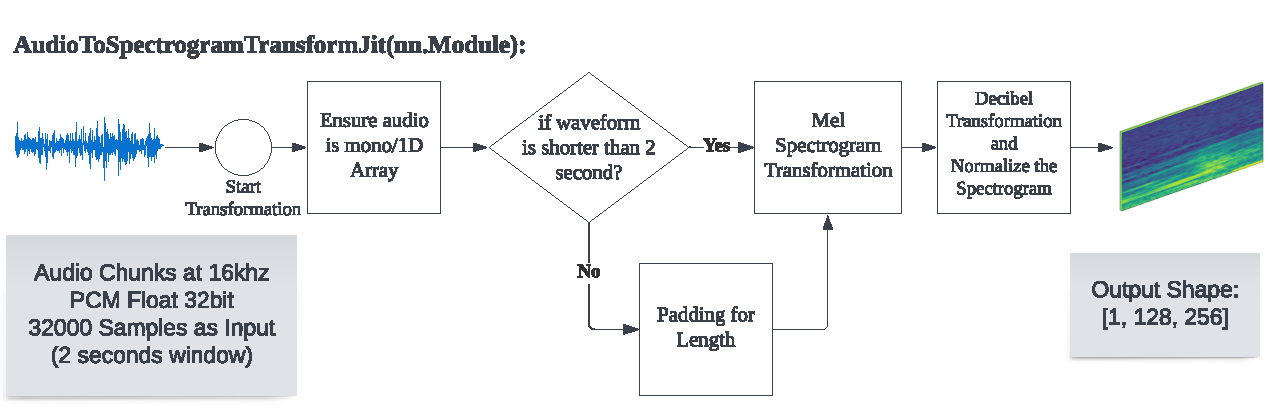
\includegraphics[width=1.0\linewidth]{img/transform.pdf}
	\caption{PyTorch Modul für die Transformation der Sprachdaten}
	\label{fig:transform}
\end{figure}


\subsubsection{Training des Modells}
Hier werden die Resultate des Trainings beschrieben. Der Datensatz wurde in Trainingsdaten und 
Testdaten aufgeteilt. Die Trainingsdaten wurden für das Training des Modells verwendet. 
Die Testdaten wurden verwendet, um das Modell nach dem Training zu evaluieren, das wird im 
Kapitel \ref{sec:evaluation} beschrieben. Die Aufteilung der Daten erfolgte mit einem Verhältnis 
von 80\% Trainingsdaten und 20\% Testdaten.

\noindent \newline
Die nachfolgenden Abbildungen zeigen verschiedene Metriken, die während des Trainingsprozesses 
aufgezeichnet wurden:

\begin{figure}[H]
    \centering
    \begin{minipage}{0.48\textwidth}
        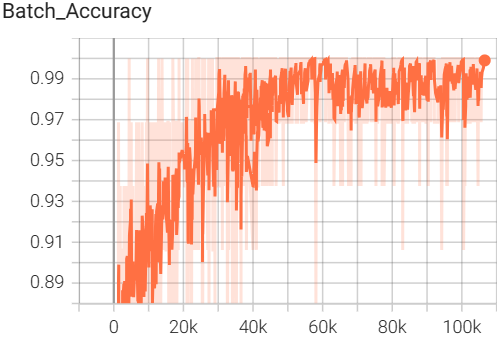
\includegraphics[width=\textwidth]{img/train/batch_accuracy.png}
        \caption{Genauigkeit pro Batch während des Trainings}
        \label{fig:batch_accuracy}
    \end{minipage}\hfill
    \begin{minipage}{0.48\textwidth}
        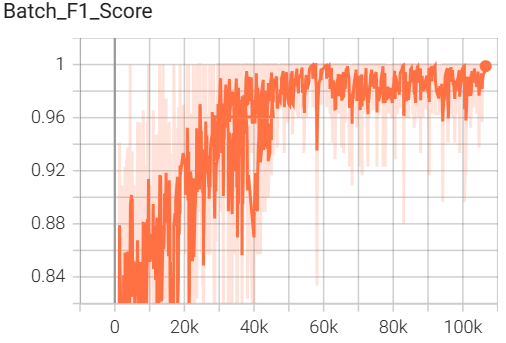
\includegraphics[width=\textwidth]{img/train/batch_f1.png}
        \caption{F1-Score pro Batch während des Trainings}
        \label{fig:batch_f1}
    \end{minipage}
\end{figure}

\begin{figure}[H]
    \centering
    \begin{minipage}{0.48\textwidth}
        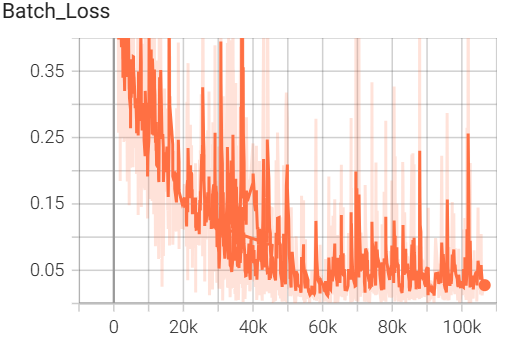
\includegraphics[width=\textwidth]{img/train/batch_loss.png}
        \caption{Loss pro Batch während des Trainings}
        \label{fig:batch_loss}
    \end{minipage}\hfill
    \begin{minipage}{0.48\textwidth}
        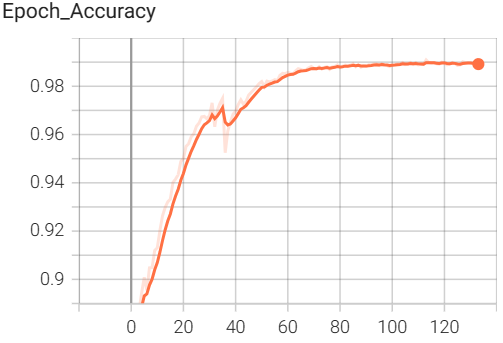
\includegraphics[width=\textwidth]{img/train/epoch_accuracy.png}
        \caption{Genauigkeit pro Epoche}
        \label{fig:epoch_accuracy}
    \end{minipage}
\end{figure}

\begin{figure}[H]
    \centering
    \begin{minipage}{0.48\textwidth}
        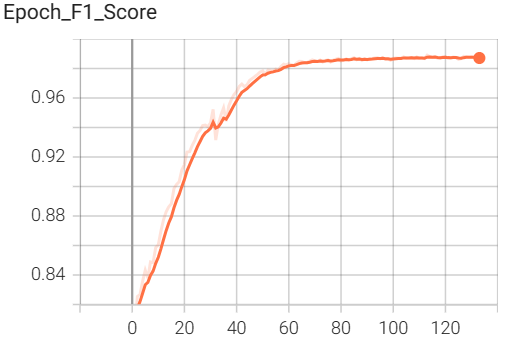
\includegraphics[width=\textwidth]{img/train/epoch_f1.png}
        \caption{F1-Score pro Epoche}
        \label{fig:epoch_f1}
    \end{minipage}\hfill
    \begin{minipage}{0.48\textwidth}
        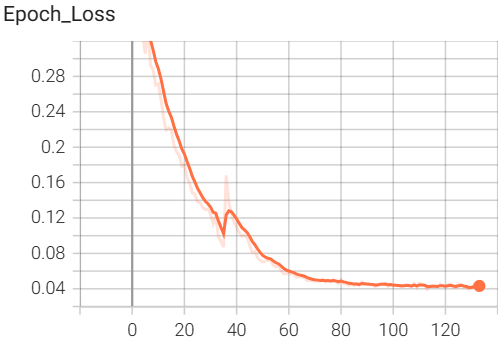
\includegraphics[width=\textwidth]{img/train/epoch_loss.png}
        \caption{Loss pro Epoche}
        \label{fig:epoch_loss}
    \end{minipage}
\end{figure}


\noindent \newline
Die Grafiken zeigen eine umfassende Übersicht über die Entwicklung der Metriken während des 
Trainings. Die Modellgenauigkeit und der F1-Score steigen kontinuierlich an, während der Loss 
kontinuierlich abnimmt. Kurz vor der 40. Epoche ist eine Unterbrechung des Trainings zu erkennen,
welche durch einen Fehler im Training Loop verursacht wurde. Es wurden fälschlicherweise bei jedem 
zweiten Sample 'Silence' hinzugefügt. Nach der Korrektur dieses Fehlers wurde das Training vom 
Punkt vor der Unterbrechung fortgesetzt, da das Modell bis dahin bereits vielversprechende 
Ergebnisse lieferte.

\subsubsection{PyTorch Scripting}
PyTorch Scripting ist eine Technik, die es ermöglicht, PyTorch-Module in ein Format zu konvertieren, 
das für die Integration in mobile Apps geeignet ist. Beziehungsweise für die Integration in die 
C++-API von PyTorch. Die C++-API von PyTorch ermöglicht die Verwendung von PyTorch-Modulen in 
anderen Programmiersprachen wie C++, Java oder Swift. Dies ist ein wichtiger Aspekt dieser Arbeit, 
da das Modell in eine mobile App integriert werden soll.

\subsubsection{Real Time Anwendung in Python}
Die Realtime Anwendung wurde in ersten Linie von (\cite{siri2017hey}) inspiriert. Dies in Bezug 
auf den Aufbau der Anwendung. Die Anwendung verarbeitet einen kontinuierlichen Audio Stream, eines 
Mikrofons. Die Verarbeitung des Audio Streams erfolgt in Stücke von 2 Sekunden. Diese Stücke werden 
alle 0.1 Sekunden verarbeitet. Zwei Sekunden sind 32000 Samples bei einer Sample Rate von 16kHz. 
Somit werden pro Sekunde 10 Inferenzen durch die Pipeline durchgeführt. Bei dieser Variante der 
Verarbeitung wird, falls das Triggerwort im Stream vorhanden ist, die Erkennung des Triggerwortes 
mehrfach erkannt. Das bietet den Vorteil einer gewissen Redundanz. Die Rate der Inferenzen könnte 
auch Variabel an die Systemleistung angepasst werden. Die nachfolgende Abbildung 
\ref{fig:realtime-application} zeigt schematisch die Realtime Anwendung. Dabei wird ein Audio Chunk 
von 2 Sekunden in ein Spektrogramm transformiert und anschliessend vom Modell verarbeitet. Das 
Resultat der Inferenz wird anschliessend in einer Progress Bar dargestellt. Die Progress Bar zeigt 
die Wahrscheinlichkeit an, dass das Triggerwort im Audio Chunk vorhanden ist. 

\begin{figure}[H]
	\centering
	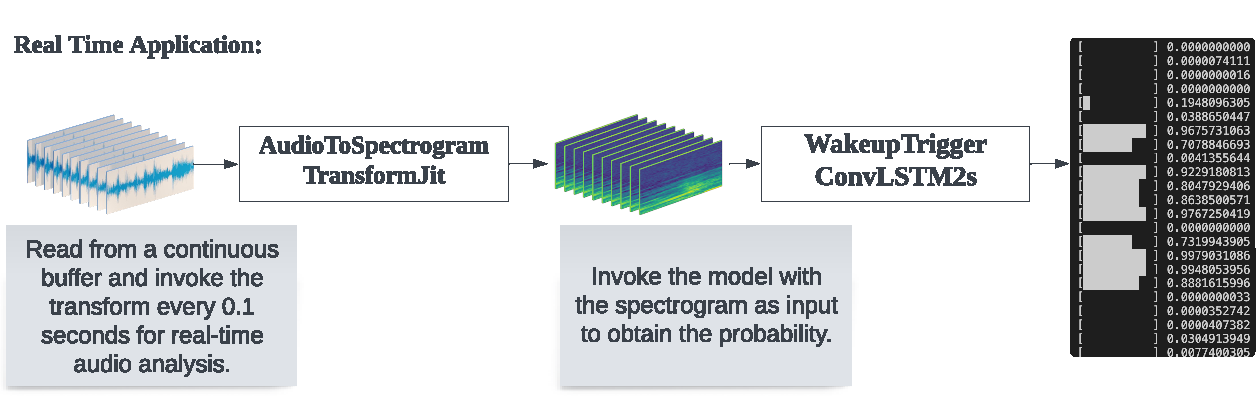
\includegraphics[width=1.0\linewidth]{img/realtime-application.pdf}
	\caption{Real Time Anwendung}
	\label{fig:realtime-application}
\end{figure}

\noindent
Mit der Ausgabe der Wahrscheinlichkeit für die verarbeiteten Audio Chunks, kann eine Entscheidung 
getroffen werden, ob das Triggerwort vorhanden ist oder nicht. Dazu wird ein Gleitender Durchschnitt 
über die Wahrscheinlichkeiten der letzten \textit{n} Audio Chunks berechnet. Ist der Durchschnitt 
über einem bestimmten Schwellenwert, wird das Triggerwort als vorhanden erkannt. Das ist auch als 
Simple Moving Average (SMA) bekannt. Die Formel für den Gleitenden Durchschnitt kann wie folgt 
beschrieben werden:

\begin{equation*}
	SMA = \frac{1}{n} \sum_{i=0}^{n} x_{i}
\end{equation*}

\noindent
Die nachfolgende Abbildung \ref{fig:sma} zeigt die Berechnung des Gleitenden Durchschnitts über 
die Wahrscheinlichkeiten der letzten 3, 5 und 10 Audio Chunks.

\begin{figure}[H]
	\centering
	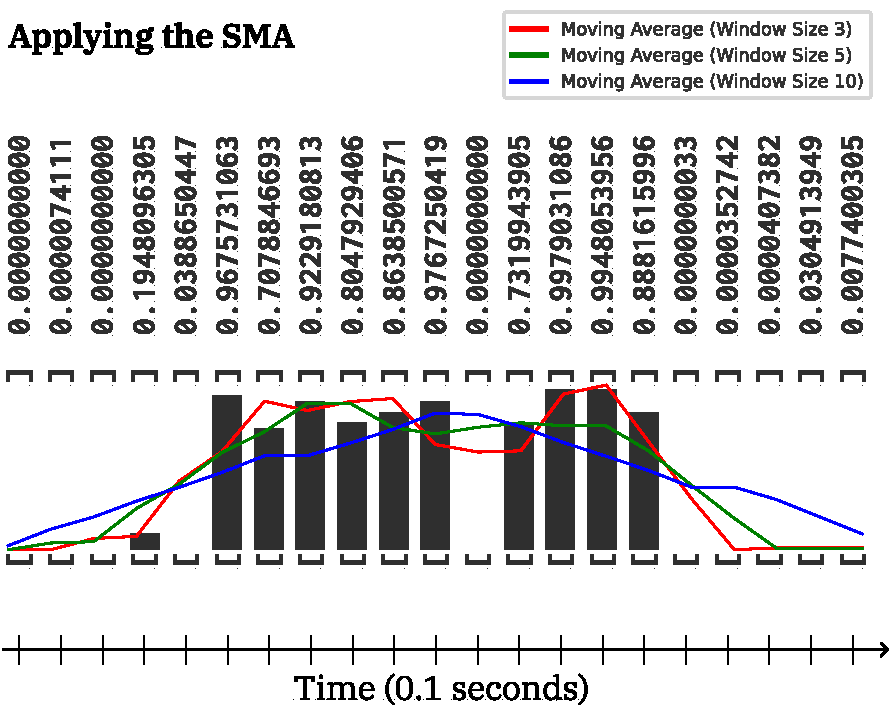
\includegraphics[width=0.5\linewidth]{img/sma.pdf}
	\caption{Berechnung des Gleitenden Durchschnitts}
	\label{fig:sma}
\end{figure}


\subsection{Integration in eine mobile App}
Im Rahmen dieser Arbeit wurde das entwickelte Modell in eine mobile Anwendung integriert, wobei die 
Entscheidung auf eine iOS-App fiel. Diese Entscheidung basierte auf der bereits bestehenden 
Vertrautheit mit der iOS-API, insbesondere \textbf{AVAudioEngine}, die im Kapitel 
\ref{sec:audio_api_integration} 'Audio API für Integration' thematisiert wurde. Die iOS-App wurde in 
Swift/Objective-C entwickelt, was eine optimale Nutzung der iOS-spezifischen Features und eine 
reibungslose Integration der PyTorch-Module ermöglichte.

\noindent \newline
Die grösste Herausforderung bei der Integration war die Anpassung der in PyTorch entwickelten Module 
für die Verwendung in der iOS-App. PyTorch Scripting spielte hierbei eine entscheidende Rolle, da 
es die Konvertierung der Module in ein Format ermöglichte, das mit der C++ API von PyTorch 
kompatibel ist. Diese Kompatibilität war essentiell für die Integration der Modelle in die mobile 
Anwendung.

\noindent \newline
Die Integration der C++ API von PyTorch in die iOS-App war ein komplexer und zeitintensiver Prozess. 
Die Herausforderung lag insbesondere in der Erstellung spezifischer Objective-C Bindings, um die 
Kommunikation zwischen der in PyTorch entwickelten Logik und der iOS-Anwendung zu ermöglichen. 
Trotz der Komplexität dieser Aufgabe wurde sie erfolgreich gemeistert, unter anderem durch die 
Nutzung von Anleitungen und Dokumentationen von PyTorch.

\noindent \newline
Während des Trainings des Modells wurden für jede Epoche Checkpoints erstellt. Für die endgültige 
Implementierung in der App wurde der Checkpoint der Epoche 120 ausgewählt. Dieser Schritt war 
entscheidend, um die bestmögliche Leistung und Genauigkeit des Modells in der App sicherzustellen. 
Für weiterführende Informationen zur Konvertierung eines PyTorch-Modells in TorchScript und dessen 
Ausführung in C++ wird auf das Tutorial \textit{Loading a PyTorch Model in C++} 
(\cite{pytorch2023jit}) verwiesen.


\newpage \section{Evaluation und Validation} \label{sec:evaluation}
Das Problem dieser Arbeit ist im wesentlichen die Erkennung von Triggerwörtern innerhalb
des Kontext einer App. Grundsätzlich ist es unüblich, dass mobile Apps eine
integrierte Sprachsteuerungsfunktion anbieten. 


\newpage \section{Ausblick}
Das Problem dieser Arbeit ist im wesentlichen die Erkennung von Triggerwörtern innerhalb
des Kontext einer App. Grundsätzlich ist es unüblich, dass mobile Apps eine
integrierte Sprachsteuerungsfunktion anbieten.

\newpage \section{Anhang}
\subfile{thesis-video.tex} % Thesis Video separat

\clearpage
% Glossar
\printglossary[type=\acronymtype,title=Akronyme]
\printglossary[title=Glossar]

% Verzeichnisse
\addcontentsline{toc}{section}{Abbildungsverzeichnis}
\listoffigures
\addcontentsline{toc}{section}{Tabellenverzeichnis}
\listoftables
\printbibliography[title=Literaturverzeichnis, heading=bibintoc]

\end{document}
